%!TEX root = ../thesis.tex
%*******************************************************************************
%****************************** Second Chapter *********************************
%*******************************************************************************

\chapter{Variation graphs}

\ifpdf
    \graphicspath{{Chapter2/Figs/Raster/}{Chapter2/Figs/PDF/}{Chapter2/Figs/}}
\else
    \graphicspath{{Chapter2/Figs/Vector/}{Chapter2/Figs/}}
\fi

Graphical models used to compress collections of genomic sequence data are unable to losslessly reproduce their own input.
This is plainly seen by considering the an alignment graph where two homologous sequences have an internal homology between them.
Such a graph will represent four possible input sequences as walks through its nodes and edges, and without additional labeling it will be impossible to obtain its input from the graph itself \cite{kehr2014genome}.

While the input sequences exist in the set of sequences that can be generated by walks through the graph, as the complexity of the graph grows the number of paths will increase exponentially.
If annotated with transition weights between nodes representing the frequency which different edges are taken by sequences in the input, then the graph can be used as an HMM to simulate new sequences.
While these will have local similarity to the graph's preimage, they are unlikely to provide a good model for the input sequences.
Sequences generated from an HMM will exhibit an exponential decay in mutual information between their symbols, while natural sequences tend to exhibit power-law decay in mutual information \cite{lin2017critical}.
This observation suggests that no pure markovian model will allow us to faithfully represent its input, and in turn that the only way to be sure that we model the input sequence space is to maintain a record of it in the context of the graph.
The compression provided by the graph is still relevant, as we can exploit the repetitive nature of natural sequences to obtain compression of this set, but using lossless techniques.

\emph{Variation graphs} (VG)\footnote{I will refer to variation graph as VG, and to the software implementation of the VG model {\tt vg}}, previously introduced in section \ref{sec:the_variation_graph}, combine a bidirectional sequence graphs with paths that model their preimage as walks through the positional space of the graph.
This makes them representationally equivalent to both graphical models and linear sequence models, and allows them to be used to model the relationships between collection of sequences, including all variation contained therein.
The encapsulation of these two divergent ways of modeling about bioinformatic data systems allows them to bridge traditionally isolated analysis modalities.
We can define these graphs by their construction from a set of pairwise alignments between sequences, as in the alignment, Enredo, and Cactus graph models, but if we want to relate new sequences to them then we would need to rebuild the entire graph to include these sequences.
By developing a model for an alignment against the variation graph we can express the relationship between new sequences and the graph without the cost of embedding the new sequence in the graph.
This allows us to follow the same kinds of analysis patterns used in resequencing, where a common reference system is used to compute a form of joint assembly between (potentially) many samples in an out of core manner.
Further, in such a scheme the reference system can remain relatively stable, which has relevance for practical use.

In this chapter, I will articulate the variation graph model and lay out the algorithms and data structures that enable its use as a reference system in pangenomic resequencing.
First I will provide formulations for the graph, its paths, edits, alignments, and genotypes define within it.
Then I will present algorithms that induce the variation graph from different data models introduced in the previous chapter.
To clarify the system's practical basis, I explain the serialization techniques used to exchange variation data.
A main focus of my work has been the efficient alignment of sequences to variation graphs.
This requires index structures to store the graph and enable queries of its topology, sequence, and path spaces, and algorithms to drive the inference of optimal alignments to the graph.
Understanding variation graphs requires techniques to visualize them, and I will present various approaches, each with particular advantages and drawbacks.
Working with variation graph references necessitates a number of mutating operations to the graph, including augmentation, sorting, pruning, and bubble simplification.
Finally, I will discuss how variation graphs can provide normalized basis spaces for the analysis of pangenomes, such as through various decompositions of alignment sets and the graph including coverage maps, ultrabubble decomposition, and haplotype matching.

\section{An extensible graphical model of many sequences}

We define a variation graph to be a graph with embedded paths $G = (N, E, P)$ comprising a set of \emph{nodes} $N = n_1 \ldots n_M$, a set of \emph{edges} $E = e_1 \ldots e_L$, and a set of \emph{paths} $P = p_1 \ldots p_Q$, each of which describes the embedding of a sequence into the graph.
At its heart, this model is simply a bidirectional sequence graph with a recorded set of walks through the graph topology.
By generalizing these paths to encode edits against the graph, we provide a mechanism to describe relations between the graph and other sequences.
Augmenting the path with additional information important to sequence analysis allows us to construct an \emph{alignment}, which forms the core data type in resequencing.
Collections of pairs of paths covering the space of two graphs describe a graph to graph alignment, or \emph{translation} which can be generated when the graph is edited to allow for the projection of coordinates and sequences in one graph into the space fo the other.
A limited form of this translation is a \emph{genotype}, which maps the implied bubble formed across multiple copies of a homologus locus in one genome into the space of the graph.
Collections of genotypes are the primary output of resequencing.
Phasing algorithms extend genotypes into longer phased haplotypes, which have a natural representation as paths through the graph.
These data models thus provide a sufficient informational basis for resequencing against variation graphs.

\subsection{The bidirectional sequence graph}

Each node $n_i$ represents a sequence $seq(n_i)$ that is built from an alphabet $\Sigma = \{ {\tt A, C, G, T, N} \}$. Nodes may be traversed in either the forward or reverse direction, with the sequence being reverse-complemented in the reverse direction.
We write $\overline{n_i}$ for the reverse-complement of node $n_i$, so that $seq(n_i) = revcomp(seq(\overline{n_i}))$.
Note that $n_i = \overline{\overline{n}}$. For convenience, we refer to both $n_i$ and $\overline{n_i}$ as ``nodes''.

Edges represent adjacencies between the sequences of the nodes they connect.
Thus, the graph implicitly encodes longer sequences as the concatenation of node sequences along walks through the graph.
Edges can be identified with the ordered pairs of oriented nodes that they link, so we can write $e_{ij} = (n_i,n_j)$.
Edges also can be traversed in either the forward or the reverse direction, with the reverse traversal defined as $\overline{e_{ij}} = (\overline{n_j},\overline{n_i})$.
Note that graphs in vg can contain ordinary cycles (in which $n_i$ is reachable from $n_i$), reversing cycles (in which $n_i$ is reachable from $\overline{n_i}$), and non-cyclic instances of reversal (in which both $n_i$ and $\overline{n_i}$ are reachable from $n_j$).

\subsection{Paths with edits}

We implement paths as an edit string with respect to the concatenation of node subsequences along a directed walk through the graph.
We do not require the alignment described by the edit string to start at the beginning of the sequence of the initial node, nor to terminate at the end of the sequence of the terminal node.
To allow the path model to support differences from the graph, each path is composed of a series of node mappings $p_i = m_1 \ldots m_{|p_i|}$ which are semantically identical to the alignment format used by standard aligners.
Each mapping $m_i = ( b_i, \Delta_i )$ has a starting position encoded as a node and offset in the graph $b_i = ( n_j, o_i )$ and a series of edits $\Delta_i = \delta_1 \ldots \delta_{|m_i|}$.
Edits $\delta_i = ( f_i, t_i, r_i )$ represent a length $f_i$ in the graph node $n_j$ (a ``from length'' in the reference), a length $t_i$ in the sequence the path encodes (a ``to length'' in the query), and encode an additional sequence $r_i$ that would replace the sequence at the given position in the reference in order to transform it into the query.
In the case of exact matches, we allow the replacement sequence $r_i$ to be empty.
They describe a function that transforms \emph{from} the graph \emph{to} the sequence.
Edits allow for rich encoding of alleles, but in practice alignments are rendered in terms of matches, mismatches, and indels.
We encode matches when $f_i = t_i \land r_i = \emptyset$, single mismatches when $f_i = t_i = 1 \land r_i \neq \emptyset$, deletions when $f_i > 0 \land t_i < 0 \land r_i = \emptyset$, and insertions when $f_i = 0 \land t_i > 0 \land r_i \neq \emptyset$.
As paths are described by a series of mappings with independent positions, they can represent all kinds of structural variation that can be represented in the bidirectional graph itself, including translocation, inversion, and copy number variation.
When mapping positions are always at the start of a node, the edit set for the path contains only matches, and the edges traversed by the path are all present in the graph, we say that the path is \emph{embedded}.
The paths from which we construct the variation graph are fully embedded, and in practice paths that contain differences occur only in the alignment of new sequences into the graph.

\subsection{Alignments}
\label{sec:alignments}

Additional auxiliary information is important when analyzing collections of DNA sequencing data sets.
Each read has a name, and an identity related to a particular sequencing experiment.
It may be related to a particular genomic sample or individual.
DNA sequence reads themselves result from a previous set of analyses run on raw observations derived from DNA, perhaps fluorescence or current traces or images.
The process of collapsing this raw information into the sequence read yields a confidence in addition to a base call.
These are recorded in a quality string in FASTQ.
The need to collect this information has resulted in the development of the SAM/BAM sequence alignment format, which provides a standard for linking the called bases (sequence), quality information, read name, features of the alignment against a reference genome and additional optional freeform annotations.

I follow this same model in developing an alignment format for read alignments to the graph.
An aligned set of sequences $Q$, $A = a_1 \ldots a_{|Q|}$, represents a sequencing experiment.
Each aligned read connects a sequence, an (optional) quality string, a path through the graph, and an optional set of $D_i$ annotations: $a_i = (s_i, q_i, p_i, k_1\ldots k_{D_i})$.
In principle the read sequence can be reconstructed from the path, but retaining the sequence information makes the alignment object lossless with respect to the input FASTQ and provides redundancy which can help in data processing.
Alignments may thus be reprocessed without reference to the graph to which they were aligned.

At their heart alignments redundantly link a sequence with a path through the graph.
They form the basis for operations on the graph, as new sequences mapped into the graph may be used to extend the graph itself by editing the graph to include the sequences represented by the alignments.
Just as alignments describe a function to edit the graph, they can describe the relationship between the sequence space of two graphs.

\subsection{Translations}
\label{sec:translation}

A generalization of the alignment is the translation set $\Phi = \phi_1 \ldots \phi_{|\Phi|}$, which relates paths in different graphs to describe the alignment between them.
A translation $\phi = (p_f, p_t)$ defines the projection between two paths which may arise in the context of two graphs $G_f$ and $G_t$.
In this use each $p_f$ corresponds to a path relative to $G_f$ (conventionally the base or reference graph), and each $p_t$ to some path in $G_t$.
However, both paths in each pair could be relative to the same graph, in which case translations allow us to descibe collections of allelic differences to the base graph.

If each node in both graphs is represened in some graph translation in $\Phi$ then it provides an isomorphic relationship between the coordinates and sequences in both graphs.
Provided each $\Phi$ encodes an isomorphism, then we can layer a series of $\Phi_i$ together to provide a coherent coordinate space across any number of updates to a given graph.
Consider a function pattern $translate$, which allows the projection of paths relative to $G_f$ through translations $\Phi$ to yield paths in $G_t$: $translate(p_i, \Phi) \to p_j \in G_t$, and similarly allows the transformation of a base graph into a target graph: $translate(G_f, \Phi) \to G_t$.
If we have a series of $(G_i, \Phi_1) \ldots (G_\rho, \Phi_\rho)$, where $translate(G_i, \Phi_i) \to G_{i+1}$ and thus each $\Phi_i$ describes an isomorphism between $G_i$ and $G_{i+1}$, then we can generate a graph translation $\Phi_\Delta$ providing $translate(G_1, \Phi_\Delta) \to G_\rho$.
We build this graph translation with the function $layer(\Phi_\alpha, \Phi_\beta) \to \Phi_{\alpha \cup \beta}$ by rewriting each path translation $\phi_i \in \Phi_\alpha$ so that its $p_t$ refers to $G_\beta$.
We do so by projecting the $p_t$ through $\Phi_\beta$, and finally adding any $\phi_j \in \Phi_\beta$ for which $p_f = \emptyset$, as these represent insertions of new sequence in $G_\beta$ relative to $G_\alpha$.

\subsection{Genotypes}
\label{sec:genotypes}

As path to path relationships can provide descriptions of allelic diversity, they form the basis for a graph-relative genotype encoding.
To represent the exact genotype of a particular sample with ploidy $\nu$ at a given locus $\iota$ we can simply collect the multiset of alleles $\pi_\iota = ( p_1 \ldots p_\nu)$.
We could alternatively build a probabilistic model $\varpi$ of an unphased genotype by using a set of $\mu$ alleles $\{ p_1 \ldots p_\mu\}$.
To do so we associate likelihoods $\gamma_\xi$ for each possible genotype $\pi_{\iota_\xi}$ that could be sampled from the alleles such that $\varpi = \gamma_1 \ldots \gamma_{\mu! \over{\nu!(\mu-\nu)!} }$.
In practice we develop our $\gamma_\xi$ out of quality information from the reads and a sampling model related to $\nu$ \cite{garrison2012haplotype,li2011stats}.
Given this definition of a genomic locus it is clear that existing genotyping models can be applied to drive genotyping using read sets aligned to the graph, and the output of the genotyper is defined fully in the space of the graph.

\subsection{Extending the graph}
\label{sec:extending}

Given an alignment $a_i$, we can edit the graph $G$ so that it includes the alignment and the sequence it represents as an embedded path, $augment(G, a_i) \to (G', \Phi)$, such that $translate(p_i, \Phi) \in G'$.
To update the path space of the graph we project all paths, including that of $a_i$, through the translation implied by the augmentation of the graph with $p_i$.
Any other $a_j$ whose path $p_j$ overlaps $p_i$ would no longer be valid, although it could be projected through the graph translation $\Phi$ as well to express it in the space of the new graph $G'$.
Updating the graph one alignment at a time is inefficient as we need to build and layer a new translation for each alignment.
It is simpler to edit the graph in a single step, taking a collection of alignments and including them in the graph, $edit(G, A) \to (G', \Phi)$.

One way to accomplish this is to first take the set of unique mappings represented in the paths of $A$, $\Omega = \{ m_1 \ldots m_{|\Omega|}\}$, and for each $m_i$ cut $n_i$ at the breakpoints where any new variation would need to be added in, adding new nodes to represent the cut portions.
Then, walking through each alignment we add in unique novel sequences and their linkages to the preexisting nodes or new breakpoints to the graph.
This process will disrupt the identifier space of the nodes and edges of the graph, but it naturally yields a translation that can be used as described in section \ref{sec:translation}.
Note that both alignments and genotypes are based on paths, so this mechanism can be used to extend the graph based on any sequence level differences that we observe either through alignment or variant calling.

\section{Variation graph construction}

We will use variation graphs as the core model for a number of essential processes in genome inference.
This model can represent many graphical sequence models used in genomics.
Each one necessitates conversion to project it into the variation graph model.
Here I describe the transformation of a number of graphical models into variation graphs, including MSAs, assembly graphs, and alignment graphs induced from pairwise alignments.
In some cases the conversion is direct, but in others it requires the addition of new labels to our model.
Variation graphs may also be built from first principles, provided a function that aligns a sequence into the graph and the editing operations described in \ref{sec:extending}.

\subsection{Progressive alignment}
%*1p 1h*
Assume a function \emph{align} that takes a sequence $Q$ and a variation graph $G$ and yields the path $p$ that is the best model of $Q$ in $G$, such that it maximizes a $\lambda$-parameterized measure $score_\lambda(p)$: or $p = \arg\max_{score_\lambda(p)} [\forall p \in G : seq(p) = Q]$.
Provided $score_\lambda$ scores exact matches above mismatches and gaps, the alignment given by $p$ will be a kind of minimal description of $Q$ in the basis of $G$.
Equivalently, it is a $\lambda$-minimal augmentation of $G$ required to include $Q$.

We can build a variation graph progressively from a set of sequences.
If we have a series of $k$ queries $q_1 \ldots q_k$, then we can build a progressive alignment by a series of edit and alignment operations applied to the variation graph.
First, take the empty graph $G_\emptyset$, to which any alignment will yield a path $p_1$ that has no mappings an which encodes the query sequence $q_1$ as a replacement sequence in the path.
We then edit the graph to add the sequence using $edit(G_\emptyset, p_1) \to G_1$.
For each subsequent $q_j$ we obtain the next graph by finding the alignment $align(q_j, G_j) \to p_j$ and editing the graph with it to yield the next graph $edit(G_j, p_j) \to G_{j+1}$ until $j = k$ and we obtain our final graph $G_{\cup \forall q_i}$.
This simple approach is attractive as it allows the variation graphs to be built from whole sequences using only techniques that are native to the variation graph model itself.
I later describe an implementation of this process multiple sequence graph alignment, {\tt vg msga}.

\subsection{Using variants in VCF format}
%*1.5p 1h*
As discussed in section \ref{sec:seq_dag_vcf}, the VCF format that is popular in resequencing implies a sequence DAG.
We can consider how to build a variation graph using the core operation $edit$.
First, we build a variation graph from the reference genome $Q_\textbf{ref}$ : $G_\textbf{ref}$.
This graph contains one path $p_\textbf{ref}$ : $seq(p_\textbf{ref}) = Q_\textbf{ref}$.
As described in section \ref{sec:genotypes} each locus reported in VCF can be encoded as a set of paths $P_\textbf{vcf} = p_1 \ldots p_V$, each representing a different one of the $V$ alleles in the VCF.
We now edit the graph to embed these allele paths, $edit(G_\textbf{ref}, P_\textbf{vcf}) \to G_\textbf{vcf}$.
Note that the graph has losslessly encoded the variant input and reference genome, and it is possible to regenerate the VCF file input by walking the positions of $p_\textbf{ref}$ and enumerating the overlapping paths as alleles in VCF format.

For efficiency, we have not implemented VCF to variation graph conversion with specifically this algorithm, but instead build up $G_\textbf{vcf}$ by walking along the reference genome $Q_\textbf{ref}$ and processing each locus independently.
This exploits the partially ordered property of the VCF to limit memory requirements when working with whole genome graphs.
For regions before, after, and between variant records at reference offsets $i$ and $j$ we add a node $n_\textbf{curr} : seq(n_\textbf{curr}) = substr(Q_\textbf{ref}, i, j)$, linking these by edges to those nodes ending at position $i$ of the reference and adding corresponding mappings for the reference path to $p_\textbf{ref}$.
At simple variant sites we add each of the alleles as a new node $n_{\textbf{var}_i}$, including an edge for each $e_{\textbf{curr} \prec \textbf{var}_i}$.
Here we also handle the reference allele differently in that we append a mapping $m_\textbf{ref} = ((n_\textbf{ref}, 0), \emptyset)$ to $p_\textbf{ref}$.
This approach seamlessly handles all kinds of common variation, including SNPs and indels, as well as more complex variation encoded as small haplotypes.

As long as the VCF records are ordered, this process allows for streaming conversion of the VCF format into a variation graph.
However, VCFs used to represent structural variation often do not describe a fully-ordered series of loci.
For instance, a large deletion may be described in one record, and followed by a number of records describing variation on the reference within the scope of the deletion.
In the graph, this results in the nesting of bubbles, and requires a deviation from a simple streaming algorithm in order to be handled.
Deletions must be recorded and linked into the downstream portion of the graph as it is later generated.
The reference allele for the deletion can only be defined once we have constructed the variation graph under the deletion.

VCFs may also encode phased haplotypes, which, like the reference, have a natural representation in the graph as paths.
Parsing these may require multiple passes over the VCF due to the memory requirements for storing large numbers of haplotypes uncompressed and cross-indexed to allow traversal in RAM.
To prevent $O(H|G_\textbf{vcf}|)$ growth of the required memory to store these, we implement efficient compression strategies on the haplotype set that exploit their repetitiveness.
There is no semantic requirement that the encoded haplotypes in VCF are valid, which introduces some complexity in the implementation of this method.
We must break haplotypes where they are found to be invalid in order to record them in VG format.
For instance, a phased VCF may report more than $\nu$ (expected ploidy) alleles for a given individual, such as when deletion and SNP variants overlap.
We expect these haplotype paths to be fully embedded in the graph an they can be represented as a walk through nodes.
Although haplotype sets are equivalent to large collections of paths, we term them \emph{threads} to indicate that they have a simpler representation than full paths.

\subsection{From gene models} % (GFF)

A reference-based RNA splicing graph is usually expressed as a set of alignments, perhaps as named intervals in BED or the General Feature Format (GFF).
As with the generic VCF generation algorithm, we can convert the transcripts to alignments $A$ relative to the graph.
Then we can then embed the transcript paths in the graph $edit(G_\textbf{ref}, A) \to G_\textbf{splice}$.
Any transcript in our set is thus encoded by the graph, and can be matched to it directly with alignment.
We also allow for novel isoforms with local similarity to the known set.

\subsection{From multiple sequence alignments}
%*0.5p 0.5h*
A multiple sequence alignment in matrix form has a simple translation into a sequence DAG and thus a VG \cite{lee2002POA}.
Given a set of sequences $Q = q_1 \ldots q_\kappa$ their $\upsilon$-long mutual alignment may be described in a $\kappa \upsilon$ matrix $X$ designed to maximize $\sum_{i=1}^{\upsilon} \sum_{j=1}^{\kappa} \sum_{k=1}^{\kappa} \delta_{X_{ij}X_{ik}}$, where $\delta$ is the Kronecker delta.
The alphabet used to encode the matrix is the same as the input sequences with the addition of a special gap character $\Box \neq \Box$, and gaps thus do not contribute positively to the matrix score.
To build a variation graph $G_\textbf{msa}$ from the MSA we proceed from $i = 1 \to \upsilon$ through $X$.
For each unique character ${\cal B}$ in the query alphabet $\Sigma \setminus \Box$ found in each row $i$, we create a node $n_{\cal B}$ in $G_\textbf{msa}$ and append a mapping to each path $p_i$ for which $n_{\cal B} \in q_i$.
We construct the edges of $G_\textbf{msa}$ by taking the distinct pairs of consecutive node traversals found in the path set $P_\textbf{msa}$ produced after the generation of the nodes in MSA traversal.
For each pair connecting nodes $n_i$ and $n_j$ we add an edge $e_{ij}$.
We can optionally compact series of nodes (which represent single characters) where no bifurcations occur, which is similar to the operation used to compact DBGs to yield unitig graphs.

Instead of a matrix, we can formulate the multiple alignment as an alignment graph (described in section \ref{sec:genome_alignment_graphs}).
By making this graph bidirectional, and thus equivalent in information content with the Enredo graph, we can see that it is equivalent to a variation graph.
Aligners that produce data formats of this type, such as Cactus \cite{Paten:2011fva}, can thus be used to produce VGs, so long as the relationship between the input sequences and the graph is recorded and can be converted into a path description.
I later use this technique to build a pangenomic reference system for a diverse set of yeast strains.

\subsection{From overlap assembly and deBruijn graphs}
%*2p 1.5h*

Overlap-based sequence graphs used in assembly, described in sections \ref{sec:overlap_graphs}, \ref{sec:de_bruijn_graphs}, and \ref{sec:string_graphs}, are nearly identical to variation graphs.
The critical difference between these models and the variation graph is that they attach a label to each edge describing the alignment between the pair of nodes which they connect.
Variation graphs do not support such a feature in their basic definition, as it is unimportant for any use of variation graphs besides temporarily representing overlap graphs.
This process is known as \emph{bluntification}, as the edges lose information and sequences given by traversing the graph are represented directly in the concatenation of node sequences.

If we reduce an overlap between a pair of nodes, it will render other overlaps on the same nodes incorrect.
Thus it is essential that the bluntification algorithm work by the reduction of sets of overlaps on edges which are transitively closed by connection to the same ends of each node, $net(e_{ij}) \to \forall e_{i*} \in G \cup \forall e_{*j} \in G$, considering both strands of the graph when doing so.
For each net we apply a function $pinch(net(e_{ij})) \to G_{\textbf{pinch}_{ij}}$, which reduces the overlaps between the nodes in the net into a blunt-edged variation graph.
We then link $G_{\textbf{pinch}_{ij}}$ back into the rest of the graph by connecting with the inbound links to each node involved in the net.
We may thus rewrite the input overlap graph as a variation graph.

In a de Bruijn graph or string graph such as SGA or Fermi2, overlaps are defined given only a length.
This simplifies the implementation of $pinch$, as no further computation is required to correctly determine the mutual alignment of overlapping sequences.
In contrast, overlaps in a generic string or overlap graph are correctly defined as alignments.
Resolving a single pairwise alignment into structures in the graph is trivial, but it becomes considerably more complex when many sequences map into a transitively closed set of overlaps.
These nets can then be resolved into an alignment graph by an algorithm similar to that given in section \ref{sec:from_pairwise_alignments}, but in practice, {\tt vg} implements bluntification by conversion of the input graph to a pinch graph library that was used to resolve the same problem in whole genome alignment \cite{Paten:2011fva}.

\subsection{From pairwise alignments}
\label{sec:from_pairwise_alignments}

Although they are mathematically equivalent, the complexity of converting various graphical genome models to variation graphs can be considerable, and {\tt vg} still lacks an ideal solution to the problem.
A set of pairwise alignments imply a variation graph, however I know of no contained method that will generate the variation graph or lossless string graph from these alignments.
One apparent problem is the memory requirements of doing so.
The full string graph for a noisy or divergent sequence set is rarely possible to maintain in RAM.
This suggest that an external memory based approach may enable greater applicability of such an approach.
To explore this, I developed an algorithm to do so that operates in external memory, which I here present in detail.
It operates by conversion of the alignment set into an alignment graph and the subsequent use of this graph in the elaboration of the variation graph including paths representing the input sequences.
The resulting graph is a lossless representation of the input and the alignments between them.
To distinguish the approach from string graphs, which imply error correction, I call this variation graph induction model the \emph{squish graph}.

% seqwish algoritm
{\tt seqwish}\footnote{\url{https://github.com/ekg/seqwish}} implements a lossless conversion from pairwise alignments between sequences to a variation graph encoding the sequences and their alignments.
As input we typically take all-versus-all alignments, but the exact structure of the alignment set may be defined in an application specific way.
This algorithm uses a series of disk-backed sorts and passes over the alignment and sequence inputs to allow the graph to be constructed from very large inputs that are commonly encountered when working with large numbers of noisy input sequences. 
Memory usage during construction and traversal is limited by the use of sorted disk-backed arrays and succinct rank/select dictionaries to record a queryable version of the graph.

%## squish graph induction algorithm

As input we have $Q$, which is a concatenation of the sequences from which we will build the graph.
We build an compressed suffix array (CSA) mapping sequence names to offsets in $Q$, and also the inverse using a rank/select dictionary on a bitvector marking the starts of sequences in $Q$.
This allows us to map between positions in the sequences of $Q$, which is the format in which alignment algorithms typically express alignments, and positions in $Q$ itself, which is the coordinate space we will use as a basis for the generation of our graph.
To relate the sequences in $Q$ to each other we apply a function $map$ to generate alignments $A$.
Although these alignments tend to be represented using oriented interval pairs in $Q$, for simplicity and robustness to graph complexity, we describe $A$ as a vector of pairs of bidirectional positions (sequence offsets and strands) $b$ in $Q$ , such that $A = (b_{q}, b_{r}), \ldots $.
We sort $A$ by the first member ($b_{q}$) of each pair, ensuring that the entries in $A$ are ordered according to their order in $Q$.

To query the induced graph we build a rank/select dictionary allowing efficient traversal of $A$, based on a bit vector $A_{bv}$ of the same length as $A$ such that we record a 1 at those positions which correspond to the first instance of a given $b_{q}$ and record a 0 in $A_{bv}$ otherwise. 
We record which $b_{q}$ we have processed in the bitvector $Q_{seen}$ which is of the same length as $Q$.
This allows us to avoid a quadratic penalty in the order of the size of the transitive closures in $Q$ given by the $map$ function.

Now we inductively derive the graph implied by the alignments.
For each base $b_{q}$ in $Q$, we find its transitive closure $c_{q} := [b_{q}, b_{r_{1}}, \ldots ]$ via the $map$ operation by traversing the aligned base pairs recorded in $A$.
We write the character of the base $b_{q}$ to a vector $S$, then for each $b_{c}$ in $c_{q}$ we record a pair $[s_{i}, b_{c}]$ into $N$ and its reverse, $[b_{c}, s_{i}]$ into $P$.
We mark $Q_{seen}$ for each base in each emitted cluster, and we do not consider marked bases in subsequent transitive closures.
By sorting $N$ and $P$ by their first entries, we can build rank/select dictionaries on them akin to that we built on $A$ that allow random access by graph base (as given in $S$) or input base (as given in $Q$).

To fully induce the variation graph we need to establish the links between bases in $S$ that would be required for us to find any sequence in the input as a walk through the graph.
We do so by rewriting $Q$ (in both the forward and reverse orientation) in terms of pairs of bases in $S$, then sorting the resulting pairs by their first element, which yields $L = [(b_{a}, b_{b}), \ldots ]$.
These pairs record the links and their frequencies, which we can emit or filter (such as by frequency) as needed given particular applications.
In typical use we take the graph to be given by the unique elements of $L$.

Our data model encodes the graph using single-base nodes, but often downstream use requires identifying nodes and thus we benefit from compressing the unitigs of the graph into single nodes, which reduces memory used by identifiers in analysis.
We can compress the node space of the graph by traversing $S$, and for each base querying the inbound links.
Maintaining a bitvector $S_{id}$ of length equal to $S$ we mark each base at which we see any link other than one from or to the previous base on the forward or reverse strand, or at bases where we have no incoming links.
By building a rank/select dictionary on $S_{id}$ we can assign a smaller set of node ids to the sequence space of the graph.

Given the id space encoded by $S_{id}$ we can materialize the graph in a variety of interchange formats, or provide id-based interfaces to the indexed squish graph.
To generate graphs in {\tt vg}  or GFA format, we want to decompose the graph into its nodes ($S$), edges ($L$) and paths ($P$).
The nodes are given by $S$ and $S_{id}$, and similarly we project $L$ and $P$ through $S_{id}$ to obtain a compressed variation graph.


\section{Data interchange}
%*0.5p 0.5h*

{\tt vg}'s design largely preceeded its development.
The mathematical concepts described in the previous section lie at the core of its implementation.
A schema language, Google Protocol Buffers (Protobuf), is used to define a compact description of data structures sufficient for the representation of all the required data models.
One cause of this pattern was my involvement in the GA4GH-DWG at the beginning of my thesis.
As the GA4GH is chartered to encourage focus on data interchange, the GA4GH-DWG was then seeking a coherent way of describing graph genomes\footnote{\url{https://github.com/ga4gh/ga4gh-schemas}} to allow support pangenomic principles resequencing.
I thus implemented the schema for {\tt vg} in the popular Protobuf schema language.
This provided a core API on which to bulid {\tt vg}.
It also implied a set of streaming data formats, which I implemented as a template library capable of serializing any stream of Protobuf objects.
Due to the reliance on Protobuf, the only code needed to implement reading and writing of these formats is {\tt vg} schema and the stream library\footnote{At the time of writing the schema, \url{https://github.com/vgteam/vg/blob/master/src/vg.proto} and stream parsing library \url{https://github.com/vgteam/vg/blob/master/src/stream.hpp} total around 1000 LOC, and are sufficient to link any C++ program into the {\tt vg} ecosystem.}.
This greatly simplified the process of developing libraries for working with the variation graph data models.
Although in practice the Protobuf data structures are slower to parse than handmade C-struct serializations like BAM, the amount of effort required to begin writing efficient and structured binary data formats was considerably less with the schema based approach.
Most importantly, the schema based definition of the core data types in {\tt vg} helped new developers and researchers using the system quickly appreciate the basic concepts.
It is not easy to measure, but I believe this has been a key cause of the success of the project and unifying many different research interests spread across many groups.

Several data formats have been important to {\tt vg}.
The graph itself can be serialized in non-overlapping chunks, where each edge $e_{ij}$ is stored once in the chunk $G_\textbf{chunk} : n_i \in G_\textbf{chunk}$.
Path mappings must have a rank that identifies their position in the path in order to be subdivided in this way, and otherwise must be serialized literally in a single vector as in GFA's ``P'' namespace.
This allows them to be read in and rebuilt even if they have been serialized out of order.
A series of alignment objects is a sensible output of the mapping algorithm {\tt vg map}.
The file format produced by writing out a series of Protobuf alignment object serializations using the {\tt stream.hpp} library is called GAM, for Graphical Alignment/Map, in analogy to SAM (Sequence Alignment/Map format).

These data models have various other equivalent serializations.
As mentioned before, the GFA format can be used to directly encode VGs, although some of the default fields (particularly the overlap CIGAR on edges) are generally not useful and carry no information.
However, GFA lacks a representation of an alignment with the same semantics as that described here.
VCF files and the reference they refer to can encode VGs, and VGs of a partially ordered format can be deconstructed into the equivalent VCF.
As paths in variation graphs can be used to represent any kind of existing annotations, data providers who represent annotations across many genomes (such as ENSEMBL Genomes) can build their annotation sets which were previously spread across many genomes into a single one embedded in a VG.
To enable this several collaborators\footnote{Jerven Bolleman and Toshiaki Katayama among others.} have developed a Resource Description Framework (RDF) compatible version of the core VG model.

\section{Index structures}

Alignment is the fundamental operation in resequencing.
Given a sequence (the ``query'') and a reference system (the ``target''), we infer a description of the query in terms of edits to the reference.
Variant calling and other genome inference problems rely on these alignments.
As described in section \ref{sec:sequence_alignment}, the large collections of read data produced by current sequencing methods require efficient read alignment to support downstream analysis.
Typically, these methods develop indexes of their reference genome, using $k$-mer hash tables or FM-index/CSA based methods capable of arbitrary-length match inference.
These indexes remain static during the resequencing analysis, and can thus be made very compact and designed to support efficient queries.
%{\tt vg} uses 

When the genome is just a linear string, distances between locations may be computed trivially, and subsets of the sequence are simply substring operations on the vector representing the genome, so no additional structure is required to seed the alignment of reads to the genome.
However, this situation changes in graphs, where the computation of distances becomes greatly more complex and particular topologies of the graph must be recorded and reproduced.
Here, I will show that graph distances may be estimated using an approximate sort and the paths embedded in the graph.
However, to do so requires efficient indexes of the path structure in the graph.
Furthermore, loading the entire graph into memory in a na\"{i}ve manner can be very expensive, and effort is required to minimize the runtime costs so as to enable resequencing even on lower-memory commodity systems.
%As with 
% summarize succinct structures for path queries

\subsection{Dynamic in-memory graph model}

Serialized in .vg or compressed GFA format, the graph of the 1000GP is not much larger than the uncompressed human reference genome.
However, the performace-oriented implemenation of the dynamic variation graph which I developed at the beginning of my studies can use a hundred times this mich memory when the entire graph is loaded into RAM.
In this scheme implemented in {\tt vg}, indexes on the node idientifier space of the graph allow for fast traversal and query of nodes by identity and neighborhood.
Various inefficiencies are accepted, such as on the hash table occupancies used to build these indexes, in the pursuit of higher performance during dynamic modification of the graph.
I now believe that it should be easy to provide a dynamic VG in low memory by using a succinct encoding, but I have not yet completed any work on this issue.
Operating on graphs of hundreds of millions of nodes with annotations like paths remains a difficult problem in this and other fields.
In most cases the graph can be subdivided (as with map/reduce processing patterns \cite{dean2008mapreduce} which underpin most industrial operation on large graphs \cite{cohen2009graph}).
This is particularly easy to implement for sequence DAG VGs, allowing for us to work on graphs of arbitrary sizes if they are approximately linear.

\subsection{Graph topology index}
\label{sec:graph_topology_index}
%*2p 3h*
While a dynamic in-memory model of a dense VG may be difficult to scale, it is comparatively easy to build succinct indexes of the graph that use only a small constant factor more memory than the uncompressed graph, yet provide support for a number of queries which are important for read mapping.

When using a variation graph as a reference system, we are unlikely to need to modify it.
As such we can compress it into a system that provides efficient access to important aspects of the graph.
Specifically, we care about the node and edge structure of the graph and queries that allow us to extract and seek to positions in embedded paths.
We would like to be able to query a part of the graph corresponding to a particular region of a chromosome in a reference path embedded in the graph.
Similarly, if we find an exact match on the graph using GCSA2, we would like to load that region of the graph into memory for efficient local alignment.

We implement a succinct representation of variation graphs in the XG\footnote{``X'' implies compression and ``G'' refers to the graph that is compressed.} library, using data structures from \href{https://github.com/simongog/sdsl-lite}{SDSL-lite}.
Node labels and node ids are stored in a collection of succinct vectors, augmented by rank/select dictionaries that allow the lookup of node sequences and node ids.
An internal node rank is given for each node, and we map from and to this internal coordinate system using a compressed integer vector of the same order as the node id range of the graph we have indexed.
To allow efficient exploration of the graph, we store each node's edge context in a structured manner in an integer vector, into which we can jump via a rank/select dictionary keyed by node rank in the graph.
Efficient traversal of the graph's topology via this structure is enabled by storing edges a relative offsets to ``to'' or ``from'' node, which obviates the need for secondary lookups and reduces the cost of step-wise traversal to member access on the containing vector and the cost of parsing each node context record that we encounter.
Paths provided to XG are used to induce multifarious coordinate systems over the graph. 
We store them using a collection of integer vectors and rank/select dictionaries that allow for efficient queries of the paths at or near a given graph position, as well as queries that give us the graph context near a given path position.

An XG index of $G = (N, E, P)$ is comprised primarily of the backing graph vector $G_\textbf{iv} = g_1 \ldots g_{|N|}$, with each $g_i$ recording the edge context for node $n_i$ in the graph: $g_i = ( \eta_i, \Xi_i)$, a sequence vector $S_\textbf{iv}$ recording the sequences labels of the nodes in a bitcompressed form, and a path membership mapping $N_\textbf{path}$.
Each $p_i \in P$ is encoded with a set of structures that allow random access of the graph by path position, which is important for the use of paths as reference coordinate systems in the graph.

To enable better compression, the node sequence space is recorded as a concatenation of node labels $S_\textbf{iv} = seq(n_i) \ldots seq(n_{|N|})$, in which each node has an offset in this sequence space defined by $seq_\textbf{offset}(n_i)$.
In bitvector $S_\textbf{bv} : |S_\textbf{bv}| = |S_\textbf{iv}|$ we set 1 at each first character in a node label, and 0 otherwise: $S_\textbf{bv}[i] = 1 \iff \exists j : seq_\textbf{offset}(n_j) = i \lor 0$.
Random access by node rank $i$ is provided by function $S_\textbf{bv}^{select_1}$, allowing us to find the sequence given a node rank in $G_\textbf{iv}$.

To allow node identifiers to be separated from the internal rank in $G_\textbf{iv}$, each context header $\eta_i$ records the external id of $n_i$.
This supports operation on subsets of larger graphs, as the subgraph retains a mapping into the node identifier space of the larger graph.

The $G_\textbf{iv}$ node context header $\eta_i$ thus links the topology of the graph to node sequences and externally resolvable node ids, as well as recording the number of inbound and outbound edges in the graph context of
$n_i$: $\eta_i = [ id(i), seq_\textbf{offset}(n_i), |seq(n_i)|, |\{e\}| : \exists e_{i*} \lor \exists e_{\overline{i}*}, |\{e\}| : \exists e_{*i} \lor e_{*\overline{i}} ]$.
Meanwhile, the edge context $\Xi_i$ enumerates the set of edges that connect to this node in a structured way that allows for oriented traversals across the two strands of the graph: $\Xi_i = \bigcup_{j=1}^{|N|} \forall e \in e_{ij}, e_{\overline{i}j}, e_{i\overline{j}}, e_{\overline{ij}}, e_{ji}, e_{\overline{j}i}, e_{j\overline{i}}, e_{\overline{ji}} : \exists e$.
To enable fast traversal we rewrite the edges in terms of relative positions in the encoded $G_\textbf{iv}$ vector, which is stored as a bitcompressed integer vector using SDSL-lite's template primitives.
Each node record is stored contiguously.
We delimit the records by a secondary bitvector $G_\textbf{bv}$, for which we build supports for functions $G_\textbf{bv}^{rank_1}$ and $G_\textbf{bv}^{select_1}$, which allow random access of $G_\textbf{iv}$ by node $id$.
Previous designs decomposed the graph structure into a set of parallel vectors, but this required multiple select queries during traversal and provided poor cache locality and performance.

Node to path membership recorded in $N_\textbf{path} = ( p_1 \ldots p_{|\{p_i : n_1 \in p_i \}|} ) \ldots ( p_{|N|} \ldots p_{|\{p_i : n_{|N|} \in p_i \}|} )$, and random access to this integer vector is provided by a rank/select dictionary built on a bitvector delimiting the various node path membership lists.
Nodes with no path membership are marked in $N_\textbf{path}$ with a 0.

Each path is represented in a set of succinct data stuctures that let us walk the path by starting at a particular node, query the path position of a given node, or find the node at a particular path position.
We store the path $p_i = m_1 \ldots m_{|p_i|}$ by decomposing its mappings into the nodes (id and orientation) it traverses $p_{i_\textbf{ids}} = id(n_j) \forall n_j \in p_i$ and $p_{i_\textbf{dir}}$ such that $p_{i_\textbf{dir}}[j] = 0 \iff m_j = (n_j, \ldots) \lor 1 \iff m_j = (\overline{n_j}, \ldots)$.
To allow rank and select queries on the node ids, we can store $p_{i_\textbf{ids}}$ in a wavelet tree, although in practice performance is greatly improved by also recording a minimum node id, so as to decrease the alphabet size of the wavelet tree, which has a large effect on WT size.
So that we may transform nodes to path positions, we use an integer vector to store a path position for each node traversal in the path, $p_{i_\textbf{pos}}$.
To go from path offset to node, we build a bitvector that marks the beginning of each node traversal in the path in a manner similar to that used to mark the sequence beginning of each node in $S_\textbf{iv}$, such that $p_{i_\textbf{offset}}$ is a bitvector of length $\sum_{j=1}^{|p_i|} |seq(p_i[j])|$ where we have marked 1 for each node start in the path, $p_{i_\textbf{offset}}[j] = \left( 1 \iff \exists n_k \in p : j = \sum_{m=1}^{k} |seq(p_i[m])| \right) \lor 0$.
By implementing $p_{i_\textbf{offset}}^{rank_1}$ we can find the node at a given path position $\mathcal{Q}$ by $p_{i_\textbf{offset}}^{rank_1}(\mathcal{Q}) \to j : \left( \sum_{k=1}^{j} |seq(p_i[k])| \leq \mathcal{Q} \land \sum_{k=1}^{j+1} |seq(p_i[k])| > \mathcal{Q} \right)$.
We can also find the position of the $j$th node in a path as $p_{i_\textbf{offset}}^{select_1}(j)$.
A CSA and rank dictionary $P_\textbf{csa}$ and $P_\textbf{name}^{rank_1}$ map from path name to internal rank of the path in $P$, which ensures maximum scalability of the path set names.

A number of compression techniques can be applied to the data models in XG to reduce the size of the overall index without any loss in functionality.
However, many of these compression methods producing compressed bitvectors, integer vectors, and wavelet trees, will result in slower access.
In the context of a short read aligner, such losses may be undesirable as long as there is sufficient memory to load the entire index into system memory, and so I have tuned the index by chosing compression strategies appropriate for its use on current datasets.

\subsection{Graph sequence indexes}
\label{sec:graph_sequence_indexes}
%*1p 2h*
Indexing the sequence space of a variation graph can be achieved using the same $k$-mer based techniques that are popular in pairwise alignment.
In the early stages of this project, I implemented a $k$-mer based index using a disk-backed system (see section \ref{sec:generic_disk_backed_indexes}).
An efficiently-built in-memory index of $k$-mers, perhaps sampled and possibly $w,k$-minimizers \cite{marccais2018asymptotically,li2018minimap2}, appears to be a reasonable basis for a sequence to graph aligner, but I did not explore this beyond these initial experiments.
Our research focus on the replication of results of the MEM-seeded short read mapper {\tt bwa mem} encouraged a similar approach for {\tt vg}.
A suffix tree provides access to a wide range of efficient sequence matching and inference algorithms, and provides a strong basis for a sensitive read aligner.

On seeing my early experiments, Jouni Sir\'{e}n, who had recently joined our lab, suggested that there might be a way to adjust his GCSA index model to work on arbitrary graphs.
He proposed a DBG transformation of the graph as input to the indexing process.
The resulting indexing model is similar to both GCSA, in its encoding of the graph topology, and succinct DBGs, which are also developed from BWTs based on a $k$-mer set.
Sir\'{e}n's design allows for the use of much longer $k$-mers than are typcially considered in DBGs, with the final DBG to be indexed having $k=256$.
As few contemparary reads are likely to generate 256bp-long sequences with no mismatch from the reference\footnote{Illumina's reads rarely reach 256bp, and when they do they tend to have higher error rates in the later cycles. The 15\% error rate of PacBio and ONT sequencing mean that a 256bp exact match is extremely unlikely, although PacBio circular consensus reads (CCR) may approach this level of accuracy.}, this approach effectively allows us to find all the SMEMs for a typical sequencing read.
The addition of the LCP array to encode the suffix tree alongside GCSA2's BWT effectively generalized all essential operations possible on a suffix tree of a string to the GCSA2, and enabled us to find SMEMs and develop sensitive MEM-based seeding heuristics using the index.
The design of GCSA2 is wholly Sir\'{e}n's work \cite{siren2017indexing}, and it forms one of the core components of the {\tt vg} mapper paper, which we coauthored.
I present it here as the mapping algorithm I developed for {\tt vg} relies on it heavily.

In broadest terms, GCSA2 employs a de Bruijn graph as a $k$-mer index of a variation graph.
Effectively the DBG nodes are labeled with their positions in the variation graph from which the DBG is generated.
To reduce redundancy, GCSA2 uses a \emph{pruned} DBG by using nodes with labels shorter than $k$ where these shorter strings still uniquely identify the beginning of their coresponding paths in the unpruned DBG.

This pruned graph is then encoded in a generalization of the FM-index built on a BWT of the $k$-mers in the pruned DBG.
The FM-index is extended to support search over the DBG by adding auxiliary bitvectors which record the indegree and outdegree of nodes in the pruned DBG.
These are used in backwards search to adjust the suffix array ranges that are considered, expanding them when the indegree is greater than 1 and contracting them when the out degree is greater than 1, in effect encoding the graph structure into the index in a space efficient and traversal optimized manner.
The technique is the same as that used in GCSA, although GCSA indexes a reverse deterministic automaton rather than a DBG.
Impressively, GCSA2 uses around 1 bit per $k$-mer in indexes of the 1000GP pangenome graph for $k=128$, which is favorable with comparsion to true DBG indexes, as these need to record information about each $k$-mer that is not important for GCSA2.

As an FM-index like structure, GCSA2 supports queries for a pattern $X$ that yield the suffix array interval matching a given pattern: $find(X) = ( sp_{X}, ep_{X} )$, and $locate( sp_{X}, ep_{X} ) = \{ b_1 \ldots b_{count(sp_{X}, ep_{X})} \}$ which yields the positions in the input VG where the given patterns occur.
The afformentioned LCP array allows the index to support several operations that require a suffix tree, including $count(sp_i, ep_i)$, which returns the number of matches for a given suffix array range, and $parent(sp_i, ep_i) = (sp_j, ep_j)$, which conceptually allows us to traverse the suffix links embedded in the suffix tree and forms the core of maximal exact match (MEM) inference using GCSA2.

GCSA2 resolves a number of problems that limit the utility of other graph path indexing schemes.
Indexing a pruned DBG allows GCSA2 to be applied to arbitrary bidirectional string graphs.
It avoids exponential costs during backwards search using the graph augmentation of the FM-index, which is itself supported by the transformation of the input variation graph into a pruned DBG.
However, it does incur exponential costs in indexing, but to mitigate the affects of these it may be constructed mostly in external memory, and furthermore construction may be broken into pieces by chromosome or some other subdivision of the graph.
Its external memory construction algorithm uses a prefix doubling approach to transform an input DBG of order $k$ to one of order $2^mk$ through $m$ doubling steps.
The high-order DBG need never be loaded into RAM but is induced from a lower-order DBG augmented with sufficient positional context on its nodes to support the disk-backed prefix doubling process.
By default, {\tt vg} runs GCSA2 with input $k=16$ and $m=4$, yielding a final DBG with $k=256$.
In indexing a DBG, GCSA2 limits the maximum-length query for which no false-positive results will be returned to the order $k$ of the DBG.
This has the benefit of allowing GCSA2 to index complex graphs, as a shorter $k$ may be chosen to limit exponential costs.
Provided the final alignment is completed against the full VG using DP-based alignment techinques that have non-exponential costs, the DBG input to GCSA2 may be constructed from a VG in which complex regions have been masked or reduced in local complexity using prior information such as a haplotype panel.

To appreciate the costs of indexing\footnote{Precise sizes are given later in the discussion of results.}, the order-256 GCSA2 may be constucted using less than 500GB of scratch space, to and from which are written approximately 3TB during construction, all while requiring less than 50G of RAM.
This puts GCSA2 indexing's resource requirements well within the specifications of standard commodity compute servers.
The resulting index occupies between five and ten times the input graph's serialized size, so no more than 50G for something in the order of a human genome.

\subsection{Haplotype indexes}
%*1.5p 3h*
% worth mentioning gpBWT and PBWT
Recording the path set of a graph in XG (described in section \ref{sec:graph_topology_index}) requires $O(N{\cal L}|P|)$ space where ${\cal L}$ is the average haplotype length, $N$ is the number of nodes in the graph, and $|P|$ is the number of paths in the graph.
Although, such a representation can be compressed, the size of this representation will grow linearly with the addition of new paths, making it impractical as a means to record very large numbers of genomes.
This encoding does simplify positional queries, but to do so each path must be stored independently and without reference to other paths.

Recording collections of paths is an important requirement for the use of VG in resequencing, as the markovian property of the bare sequence graph $G = (N, E, P= \emptyset)$ means it can encode exponentially many paths relative to the true input path set used to build the graph.
This introduces significant issues during read mapping and genome inference.
With increasing variant density the number of haplotypes grows exponentially, and this can lead to spurious mismapping as discussed in section \ref{sec:1000GP_sim}.
The exponential growth of the path space of the graph has relevance for sequence indexing with GCSA2, and as described in \ref{sec:graph_sequence_indexes}, simplification of the graph input to GCSA2 indexing is required to reliably build indexes.
A haplotype index is the only way that the pruning operation applied to the graph may preserve known haplotypes, rather than defaulting to the reference genome in such cases.
Efficient path indexes could be used for many operations in variant calling and phasing, and may have utility in assembly problems, for instance to losslessly record a read set embedded in a squish graph representing their mutual alignment (section \ref{sec:from_pairwise_alignments}).

Haplotypes from the genomes of the same species are often shared exactly, which suggests that they may be very efficiently compressed.
This property was first used to store large haplotype sets in the \emph{positional BWT} (PBWT) \cite{durbin2014efficient}.
As input the PBWT assumes a set of haplotype strings $S_1 \ldots S_m$ of the same length which describe a set of haplotypes relative to a set of variable loci.
$S_j[i]$ records the allele in haplotype $j$ found at locus $i$.
We set $S_j[i] = 0$ when haplotype $j$ has the reference allele at locus $i$, and $S_j[i] > 0$ if it encodes one of possibly several alternate alleles.
The PBWT can be understood as an FM-index of texts $T_1 \ldots T_m : T_j[i] = (i, S_j[i])$ \cite{gagie2017wheeler}.
To search for a haplotype of $h$ in the range $[i,j]$ we look for pattern $h' = (i, h[1]) \ldots (j, h[|h|])$.
The alphabet size of this FM-index is large, but the matrix like structure of the haplotype set means that we can implicitly encode the array indexes by building a separate sub index for each position.
Applying run length encoding to the BWT allows extremely good compression of real haplotype sets.

With the \emph{graph positional Burrows–Wheeler transform} (gPBWT) \cite{Novak2016gPBWT}, we extended this model to work on variation graphs.
The basic model is the same as the generic PBWT except that instead of variant matrix positions we consider haplotype traversals of node ``sides'' $n_i$ or $\overline{n_i}$, and rather than a local alphabet of variant alleles we encode a local alphabet $\Sigma_{n_i} = \{ j \in N | e_{ij} \in E \}$ which describes the set of nodes $n_{\{j \in N | e_{ij} \in E \}}$ to which haplotypes go after the current node (side) $n_i$.
As in the generic PBWT we build an FM-index of $T_1 \ldots T_m$, encoded in what we call the $B_s$ arrays, which provide the local description of prefix sorted haplotypes (equivalently, threads) traversing each node side $n_s$.
To deal with bidirectionality of paths in variation graphs, each haplotype must be encoded in its forward and reverse orientation.
We demonstrated the expected sublinear scaling property for the gPBWT by building an index for chr22 with increasing numbers of samples.
Constructing the gPBWT for large haplotype sets proved difficult when using our particular implementation.
Progressive construction of the gPBWT in generic graphs was enabled by encoding the gPBWT into dynamic succinct data structures and adding a single haplotype thread and its inverse one at a time.
The overheads associated with the dynamic succinct data structures and the linear time required resulted in an infeasible serial construction algorithm for large haplotype sets, and all experiments were carried out using a partially ordered construction algorithm that worked using a VCF file as input.

The \emph{graph Burrows-Wheeler transform} (GBWT) \cite{siren2018haplotype} simplifies the data model used by gPBWT so that it is independent of {\tt vg} and can be applied to generic sequence graphs.
The most generic conceptual model for the GBWT is as the FM-index of a transformation of the graph's paths $p_1\ldots p_m \cup \overline{p_1}\ldots \overline{p_m}$ into the text $T = \$( p1 = n_i\ldots n_j) \ldots \$ (\overline{p_m} = \overline{n_j} \ldots \overline{n_i}) $ wherin the paths are rewritten as a series of characters representing node traversals in a large alphabet and delimited by a marker $\$$.
Unfortunately, this approach is technically challenging to implement due to the extremely large size of $T$ for moderately-sized haplotype sets embedded in variation graphs ($|T| \approx 10^{12}$ for the 1000GP  \cite{siren2018haplotype}).
Serializing the path set during construction is not feasible, which suggests a dynamic version of the model is required.
Also this approach it does not benefit from a number of features which distinguish paths in typical variation graphs.
Sequence graphs based on homology tend to be manifoldly partially ordered, as unique sequence will easily assemble into long coherently-ordered segments.
If we sort the identifier space of these graphs, then most haplotypes passing through the graph will be comprised of increasing or decreasing sequences.
This is even more true for VGs built from VCFs, although even there the issue of indels must be handled in a way that is very different from the assumptions that simplify the PBWT.
The nodes in these regions of the graph will also tend to have low degree.
These features suggest that a local compression of each's node's context in the graph can be achieved very efficiently.
The GBWT can thus benefit from a formulation in similar positional terms as those used in PBWT, with the augmentation of the positional model to record its local context in the graph.
The isolation of each node's context can also allow the construction of the GBWT to be completed in parallel over isolated segments of the variation graph, such as separate chromosomes, and these may be merged easily.

In the GBWT we break the full FM-index into per-node records, each of which encodes a header consisting of a description of the local edge transition alphabet $\Sigma_{n_i}$ through which the graph topology is maintained, and a body $BWT_{n_i}$ which is the subset of the full BWT specific to paths traversing $n_i$.
The GBWT supports essential FM-index operations including: $find(X) \to [sp, ep]$ yielding the lexicographic range of suffixes starting with pattern $X$; $locate(sp, ep) \to$ paths occuring in $SA[sp, ep]$; and $extract(j) \to p_j$ which returns the $j$th path in the graph.
By encoding all paths in both orientations, the GBWT can be treated as a kind of FMD-index for haplotypes, allowing bidirectional search.
In principle, this means that the GBWT turn supports MEM-based haplotype matching, which has potential uses in genotype imputation, phasing, association mapping, and other population genetic and evolutionary assays.

The GBWT representation reflects a number of assumptions that tend to hold for most DNA sequence graphs.
Nodes tend to have low degree, which means the local alphabet size $|\Sigma_i|$ is small and we can afford to decompress a local alphabet encoding efficiently.
Most nodes are not traversed more than once by each path, so the $BWT_{n_i}$ remains small and can be accessed and modified in bounded time.
Due to relatedness among individuals in many species, it is sensible to assume that haplotypes will be highly repetitive, which allows for efficient RLE encoding of $BWT_{n_i}$.
The graph is sorted, and its identifier space has been compacted, which allows us to store the same information for the entire range of node identifiers in bounded memory with respect to $|N|$.
The graph tends to be locally ordered in most cases, which decreases the complexity of recording the graph topology in our records.

%GBWT builds an efficient dynamic model 

%To resolve the issues with construction faced by gPBWT, GBWT 

A \emph{dynamic GBWT} implementation presents the node records through an index over the range of $[min(i : n_i \in N), max(i : n_i \in N)]$, for each linking to its header, body, incoming edges, and haplotype identifiers.
Construction employs this model in a manner similar to RopeBWT2 \cite{li2014fast}, where batches of paths are insert into the index in a single step following the BCR construction algorithm to build the BWT for large sequence sets \cite{bauer2013lightweight}.
This process includes the new paths in the dynamic GBWT by rebuilding each node record affected by the extension.
At the end of each step the dynamic GBWT remains valid.
When constructed, the GBWT may be encoded in a compacted but immutable form that uses less memory.
By breaking the construction process apart for each chromosome and finally merging the compressed GBWTs, it is possible to build the GBWT for the entire 1000GP haplotype set around 30 hours.
The resulting GBWT requires $\approx 15$GB, with around half allocated to the GBWT structure itself and half to haplotype identifiers.
Incredibly, this structure requires less than 0.1 bits per mapping in the stored paths.
This demonstrates that it has fully exploited haplotype sharing in the 1000GP set, and we can expect that this compression rate will only improve with the addition of more samples.

\subsection{Generic disk backed indexes}
%*0.5p 0.5h*
\label{sec:generic_disk_backed_indexes}
I began the development of {\tt vg} alone, starting with schemas for the data models, then building an index of the graph using the disk-backed key/value store RocksDB\footnote{\url{https://github.com/vgteam/vg/blob/master/src/index.hpp}}.
In principle this would allow working with graphs that were many times larger than main memory.
I transcribed the data model into namespaces and sorted arrays written into the key/value store.
As compressors of various types could be applied to the sorted arrays backing RocksDB, the memory uses of this approach were ultimately similar to those for the final indexing models that I present here.
This encoding included the graph, alignments, and 
However, performance was far worse and the initial version of the aligner based on these systems could not achieve meaningful results using reasonable amountsof time for large graphs.
Ultimately, this flexible database model has remained important for some pipelines, in particular as a technique to organize alignments against the graph.
The ability of a disk backed index to exceed main memory limits makes it useful for exactly this kind of workload.
Unfortunately, other workloads such as sequence queries were untenable for large genomes, with reliable performance only possible if the entire index of spaced $27$-mers were cached in RAM, requiring nearly 200G in the case of the 1000GP variation graph.
The sorted disk-backed array does have the useful property of allowing prefix queries of the $k$-mer set, but this can easily be attained with GCSA2.
Finally, on the networked storage available in my instutitional setting, the construction costs for disk-backed index models were usually much worse than those of the XG and GCSA2 models.

\subsection{Coverage index}
\label{sec:coverage_index}

As variation graphs can remove specific bias towards any particular sequence, they imply a uniform vector space in which all samples can be placed for later analysis.
One reductive form that this can take is a coverage map, which is similar to the labeling required to implement ``colors'' on a DBG.
Here, we lose information about the edge traversals and the paths taken through the graph
In principle, this doesn't matter for many kinds of variation.
And in benefit,, but the complexity of computing the coverage map is linear in the number of the input alignment set, and it requires $O(\sum_{\forall{n_i\in N}}|n_i|)$ space.
In exploration of this, I developed an indexing method that allows us to build and query compact coverage indexes.
Simply, we map the sequence space of the graph into a vector and record coverage across it for a GAM read set.
During construction, a succinct format is employed to store the coverages in a single byte as long as they are below 255, and in a secondary hash table if they reach 256.
Finally a compressed integer vector is generated, which be queried by graph position computed from the XG index of the graph.
I extended this concept with a kind of succinct ``pileup'' format \cite{li2009sequence} generated from the edits against the graph.
In this model edits in mappings which don't match the reference were serialized into a byte alphabet using protobuf, such that each non-reference edit $e_j$ at position $b_i$ was recorded as a string $\$b_i e_j$, and these were combined and delimited by a character $\$$ escaped from the representation by duplication of all instances in the byte string.
By building a CSA/FM-index from these I can obtain the set of edits at each graph position through pattern matching.
However, I found it impossible to construct this for a large high-coverage sequencing sample, and have not continued research into the topic.

\section{Sequence alignment to the graph}
%*0.5p 0.5h*
We have built variation graphs to be used as a pangenomic reference for sequence analysis.
The most important step in such analysis is sequence alignment.
Aside from whole genome alignment methods, which implicitly use such techniques, no previously published approach allows the sensitive alignment of long sequences to large graphs.
The graphs we build are meant to encode any kind of variation.
Our alignment algorithm should be able to represent them in alignments as well.
I have explored a particular hierarchical model of alignment that does by using hierarchical partial alignment of the sequence to the graph.
In \emph{chunked alignment}, large sequences are broken up into overlapping segments, each of which is aligned individually in any order or orientation.
This subdivision provides a kind of banding to the alignment algorithm, preventing the evaluation of the full DP matrix, but more importantly it also allows alignments that are generated to represent any kind of variation.
Each chunk is aligned indepenently using one of several possible algorithms.
I use GCSA2 and the XG index to find and cluster maximal exact matches (MEMs) using a global pseudoalignment algorithm that exploits approximate distance indexes in the graph to drive colinear chaining of MEMs.
The same colinear chaining model, with different parameters, is used to establish the optimal global chain through the alignment chunks, thus yielding a full alignment for the input sequence of any size.
In the simple case where our reads are shorter than the standard chunk size (256bp), the alignment behaves exactly as in {\tt bwa mem}, and this use constitutes much of the application of the method in the subsequent chapter.
Locally, I use a SIMD-accelerated dynamic programming approach that generalizes Smith Waterman Gotoh (SWG) to operate on a graph to align each chunk to each candidate locus.
\emph{Unfolding} and \emph{DAGification} transform a cyclic bidirectional sequence graph with inversions to an acyclic simple sequence graph one in which all $k$-paths in the first graph are represented.
Any alignment algorithm that may be implemented on a sequence DAG can thus be used.
Optionally, other alternative DP alignment algorithms implementing a banded global alignment can be applied, and I also report on these as I have supported their authors' implementation of them in {\tt vg} and used them in related algorithms such as the \emph{surjection} of alignments into a particular reference path.

\subsection{MEM finding}
%*2p 2h*
{\tt vg} can efficiently align reads against large graphs supported by xg and GCSA2 indexes through an alignment process based on maximal exact match sequences between the query sequence and the reference graph.
First, a set of super-maximal exact matches (SMEMs) of a read are generated by traversing the suffix tree encoded in the GCSA2 index until the count of matching strings drops to 0, then backing off one step to find all longest exact matches. 
A recursive series of ``reseed'' passes through the traversal can then identify next-longest matches which are used both to improve sensitivity.
These are not super-maximal, thus we tend to call these heuristically derived exact matches ``MEMs''.
Then, chains of MEMs that are consistent with the query sequence are found using a Markov model in which the optimal alignment is likely to form a Viterbi path.
For each candidate chain, we then locally align the read against the graph. 
Scoring results from the local alignment are used to rank the candidate alignments.
We then return the best alignment, or multiple candidates if multiple mappings are required.

\subsection{Distance estimation}
%*1p 1h*
To cluster our MEMs we require a distance function that returns the minimum distance between any two positions $dist(b_i, b_j) \to \min_{\forall p \in N \times N}{|p|} : pos(p[1]) = b_i \land pos(p[|p|]) = b_j$.
Distance measurement between nodes in a variation graph is non-trivial, with exact solutions to the problem theoretically requiring $O(E \log \log L)$ where $L = \max_{\forall n_i \in N} |n_i|$ is the maximum node length \cite{karlsson1983mlog}.
Precomputation of the full set of distances would thus require $O(N^2 E \log \log L)$ time and $O(N^2)$ space, which is infeasible for any large graph.
Many variation graphs are mostly linear, which we can exploit to build an approximate distance metric.
Provided we have applied a partial sort to the graph, in the partially ordered regions we can use the offset of each node in the XG sequence vector $S_\textbf{iv}$ as approximate 1D coordinates for each node.
We expect that in much of the graph $S_\textbf{bv}^{select_1}(id(b_j)+offset(b_j)) - S_\textbf{bv}^{select_1}(id(n_i)+offset(n_i)) \propto dist(b_i, b_j)$, where $id(b)$ is the function that returns the rank of position $b$'s node in the XG index, and $offset(b)$ returns the position's offset inside the sequence label of the node.
We use this to provide a first order approximate distance metric.
Nonlinearities in the graph will frustrate this metric, and to manage these we rely on the positional index provided by the \emph{positional paths} given in the XG index.
In these, we can query the relative positions of nodes in the path in $O(1)$ time.
Where both positions are not on the same path, we can use local exploration of the graph near our positions $b_i$ and $b_j$ to attempt to find anchoring nodes on the same path.
In our clustering step we can consider the multiple coordinate systems to develop a global pseudoalignment.

\subsection{Collinear chaining}
%*0.5p 0.5h*
\label{sec:collinear_chaining}

If the MEMs do not cover the full read length then we attempt to link them together into chains by building a Markov model in which the best possible chains form high-scoring paths. 
In this model the nodes correspond to the reference graph positions where MEMs in the read occur and the transitions between nodes correspond to a weight that is proportional to the indel size implied by the difference in distance between the positions of the MEMs in the read and their approximate or embedded path-relative distances in the graph. 
To consider the coordinate spaces implied by all applicable embedded paths, we record one node per embedded path that each MEM touches. 
We also record a node for each MEM based on its approximate position in the graph, which is estimated as its position in the concatenated nodes of the partially sorted graph. 
If we are aligning a read pair, the weight between MEMs on different fragments is proportional to the probability of that distance under a learned model of the fragment distribution. 
One we establish this model, we take the Viterbi path through it as our first candidate alignment. 
By masking this path out and re-running the Viterbi algorithm on the model, we can extract a series of candidate alignments in descending order of goodness. 
This clustering model implements a kind of co-linear chaining such that optimal chains are made of series of MEMs which have similar spacing in the read and in the reference system into which we are mapping the read. 
Although the exact algorithm is different, in spirit our implementation is similar to that developed in \cite{kuosmanen2018using}, which extends colinear chaining to DAGs by running a similar model over the paths in a minimum path cover which they efficiently compute on the graph.

\subsection{Unfolding}

Every node has an implicit default orientation (see Graph Representation below) so that it is possible to determine edges that cause an inversion, i.e. those which connect between a forward and a reverse complement node orientation. 
In {\tt VG::unfold} we use a breadth first search starting at every inverting edge in the graph to explore the reverse complemented portions of the graph that we can reach within length $k$ from the inverting edge.
We then copy this subgraph, take its reverse complement, and replace the inverting edges connecting it to the forward strand of the graph with non-inverting ones.
If $k$ is greater than any length in our graph, then we are guaranteed to  duplicate the entire reverse complement of the graph on the forward strand, effectively doubling the size of the graph if we have any inversions in it.%, as shown in Supplementary Figure 3. %\ref{fig:unfold}.

\subsection{DAGification}
\label{sec:DAGify}

Variation graphs may have cycles.
These are useful as compact representations of copy number variable regions, and arise naturally in the process of genome assembly.
However, our partial order alignment implementation does not handle these structures, and so when they occur we convert them into an $k$-path equivalent acyclic graph in order to align with DAG-based alignment algorithms.
To do so, we unroll cyclic structures by copying their internal nodes an appropriate number of times to allow a given query length to align through the unrolled version of the component.
In this graph, we can find all paths of length $k$ found in the original graph.
If our query is shorter than this limit, $k \geq |Q|$, then we are guaranteed to find the optimal alignment in the original graph by aligning against the DAGified one.

We first detect all strongly connected components by using a recursion-free implementation of Tarjan's strongly connected components algorithm \cite{tarjan1972depth}.
Then, we copy each strongly connected component and its internal edges into a new graph.
We greedily break edges in this graph that introduce cycles.
Next we k-DAGify the component progressively copying the base component and, for each edge between nodes in the component, connecting from the source node in the previous copy to the target node in the current copy.

We use dynamic programming to track the minimum distance back through the graph to a root node outside the component at each step.
When this reaches our target $k$, we stop unrolling, and add the expanded component back into the graph by reconnecting it with its original neighborhood.
For each copy of a node in the DAG-ified component we copy all its inbound and outbound edges where the other end of the edge lies outside the strongly connected component.
The resulting graph is acyclic and supports queries up to length $k$ on the original graph using the translation that we maintain between the new graph and the source one.
%Figure \ref{fig:kdagify} 
%Supplementary Figure 4 provides a visual description of the process.


\subsection{POA and GSSW}
%*2p 2h*

Partial order alignment (POA), which I previously describe in section \ref{sec:MSA}, generalizes string to graph and graph to graph alignment for the case of sequence DAGs.
It is the core alignment algorithm used in {\tt vg map}.
Where POA was defined for graphs in which each node represents a single base, we must account for the compressed nature of variation graphs, which adds some complexity in our definition and implementation.
Furthermore, default POA is efficient in terms of runtime, but does not benefit from vectorized instructions that are now ubiquitous on modern processors.
As part of work in the 1000GP, I developed an accelerated version of POA which I will present in detail here.

Given a candidate cluster of exact matches that we have extracted from the MEM chaining model described in the previous section \ref{sec:collinear_chaining}, we want to derive a complete description of the alignment of the read to the reference graph.
Sensitive alignment of each candidate is essential for distinguishing the optimal alignment.

We transform seed chains into alignment using local alignment based on dynamic programming. 
To make this efficient we extended an implementation \cite{zhao2013ssw} of Farrar's SIMD-accelerated striped Smith Waterman (SSW) algorithm \cite{farrar2007striped}, which we term \emph{graph striped Smith-Waterman} (GSSW)\footnote{\url{https://github.com/vgteam/gssw}}.
Single-Input Multiple-Data (SIMD) instructions allow vectorized mathematical operations in a single machine instruction, and can be used to greatly speed up algorithms which can be implemented in terms of operations on vectors.

GSSW generalizes all aspects of SSW to operate over sequence directed acyclic graphs, including affine gap penalties, and retains its matrices for traceback\footnote{SSW discards these matrices for performance reasons, instead establishing the traceback later with local banded DP.}.
This is simple to accomplish if the reference is a graph, as the striping of SIMD calculations in SSW across the reference is done by a single character at a time, and thus boundaries between nodes do not split the SIMD embedded variables.
We can generalize SSW to GSSW by extending the recurrence relation that defines the scores in the DP matrices to consider all previous positions on all nodes that connect to the current one.

Given a query $Q$ and a sequence graph $G = (N, E)$ with sequence length $L=\sum_{i}^{|N|} |seq(n_i)|$.
We record the maximum scores of alignments between $Q$ and $G$ in the tensor $\hat{\cal H} = {\cal H}_1 \ldots {\cal H}_{|N|} :$ each ${\cal H}_i$ is a $|seq(n_i)| \times |Q|$ matix.
$\hat{\cal H}$ thus contains $|Q|\times L$ cells, and when we have completed the scoring phase of alignment each will record the maximum score of an alignment between $Q$ and $G$ ending at $(n_i[x], Q[y])$ in ${\cal H}_{i}[x,y]$\footnote{Here I will use brackets $[\ldots]$ to identify the cells in 2-dimensional arrays.}.
To develop our scores, we use a scoring function $score(a, b)$, which in the case of DNA returns the value of a match (typically a positive integer) when $a = b \lor a = N \lor b = N$ and the value of mismatch when $a \neq b$ (typically a negative integer).
We score a gap beginning with $\omega_\textbf{open}$ and a gap extension as $\omega_\textbf{extend}$
We record the score of a gap along $G$ in tensor $\hat{\cal E} = {\cal E}_1 \ldots {\cal E}_{|N|}$ and a gap along $Q$ in tensor $\hat{\cal F} = {\cal F}_1 \ldots {\cal F}_{|N|}$.

Gaps in $\hat{\cal E}$ extend across the graph, and so we need to consider all the inbound edges when we are at the beginning of a node:

\begin{equation}
  {\cal E}_i[x,y] = \max
  \begin{cases}
    {\cal E}_i[x,y-1] - \omega_\textbf{extend} \\
    {\cal H}_i[x,y-1] - \omega_\textbf{open} \\
    \max_{\forall j : \exists e_{ji} \in E} {\cal E}_j[|n_j|,y-1] - \omega_\textbf{extend} & \text{if } x = 1 \\
    \max_{\forall j : \exists e_{ji} \in E} {\cal H}_j[|n_j|,y-1] - \omega_\textbf{open} & \text{if } x = 1 \\
  \end{cases}
\end{equation}

However, this is not the case for $\hat{\cal F}$, whose data dependencies flow vertically over the query $Q$:

\begin{equation}
  {\cal F}_i[x,y] = \max
  \begin{cases}
    {\cal F}_i[x-1,y] - \omega_\textbf{extend} \\
    {\cal H}_i[x-1,y] - \omega_\textbf{open} \\
  \end{cases}
\end{equation}


The score in $\hat{\cal H}$ combines the affine gap calculations in $\hat{\cal E}$ and $\hat{\cal F}$.
As with $\hat{\cal E}$, we here we also must consider the inbound nodes:

\begin{equation}
  \label{eqn:gssw_h}
  {\cal H}_i[x,y] = \max
  \begin{cases}
    0 \\
    {\cal E}_i[x,y] \\
    {\cal F}_i[x,y] \\
    {\cal H}_i[x-1,y-1] - score(Q[x], n_i[y])\\
    \max_{\forall j : e_{ji} \in E} {\cal H}_j[|n_j|,y-1] - score(Q[x], n_j[y]) & \text{if } x = 1 \\
  \end{cases}
\end{equation}

The values of ${\cal H}_i$, ${\cal E}_i$, and ${\cal F}_i$ are 0 when $x < 1$ or $y < 1$ and node $n_i$ has no inbound edges.
Note that this is the initial condition provided by Gotoh to improve the algorithm of Smith and Waterman.

We fill the matrices using Farrar's SSW algorithm \cite{farrar2007striped}, based on Zhao's implementation \cite{zhao2013ssw}.
By storing the full score matrices we can then trace back from the maximum score in $\hat{\cal H}$ to obtain the optimal alignments under our scoring parameters.
The traceback can be represented as moves in the matrix, or equivalently as the alignment object model described in section \ref{sec:alignments}.

To interface with GSSW we transform a local region of our graph so that it is acyclic and only represents a single strand of the DNA as described in section \ref{sec:DAGify}.
The two operations we use in this transformation are \emph{unfold}, which expands the graph to include its reverse complement where accessible via an inversion, and \emph{dagify}, which unrolls strongly connected components of the graph far enough that we are guaranteed to be able to find any sequence of given length $k$ in the source graph in the unrolled one.
This allows us to align any sequence of up to length $k$ against a completely general section of a variation graph.
Through these steps we retain a mapping from old node ids to new ones, which we will use to project alignments to the transformed graph back into our base coordinate space.

\subsection{Banded global alignment and multipath mapping}
\label{sec:banded_global}

By modifying equation \ref{eqn:gssw_h} so that it is no longer capped at 0 and changing the traceback so that it goes from beginning to end of query $Q$ and graph $G$, we obtain a ``global'' alignment algorithm with the same properties as Needleman-Wunsch.
The SIMD-based approach of GSSW is not adapted to negative scores, and so the implementation of global alignment to the graph is completed a standard DP approach as in POA.
However, it may be \emph{banded} so that only a limited region of the DP tables need to be explored.
This approach, as implemented in {\tt vg} by Jordan Eizenga, forms the basis for multipath mapping, in which alignments are represented probabilistically as DAGs rather than linear series of node traversals and edits.
In multipath mapping, regions between MEMs in a particular cluster may be aligned using global alignment, so as to obtain full-length descriptions of the alignment in the non-matching region.
Multiple traceback allows for alternatives to be included, and each of these may be scored on the basis of both alignment score and haplotype matching score.
His implementation is key to the development of haplotype aware mapping, which is the subject of a paper currently in development by collaborators on the {\tt vg} project.
In the case of low-error reads, this limited exploration of the DP problem allows for fast derivation of the optimal alignments, and so the multipath mapper in {\tt vg mpmap} achives runtime comparable to or exceeding the simpler algorithm in {\tt vg map}.
It is also important to mention here as it forms the basis for alignment surjection, in which an alignment to the graph is projected into the linear reference.

\subsection{X-drop DP}

As our query length $|Q|$ increases, so does the practical complexity of deriving the alignment using POA/GSSW.
Given that we tend to align against proportionally larger graphs and so we effectively face a quadratic penalty with increasing alignment length, $|Q| \propto |L| \implies$ GSSW is $O(|Q|^2)$.
The most direct solution to this is to use a banded alignment method like banded global alignment, as described in section \ref{sec:banded_global}.
However, this method cannot exploit data parallel operations that allow dramatic speedups on modern processors.

In the course of our work on {\tt vg}, Eizenga and I explored the application of Hajime Suzuki's adaptive banded global alignment (libgaba)\footnote{\url{https://github.com/ocxtal/libgaba}} \cite{suzuki2017acceleration}, which has been used in to greatly improve alignment speed with long single-molecule reads \cite{li2018minimap2}.
In this approach, an antidiagonal band of cells are computed at each step, of a predetermined width designed to fit into the word sizes of SIMD instructions.
The band can move either ``right'' or ``down'' at each step, depending on where the highest score is found.
A termination criteria is given, so that alignment stops when the maximum score falls a given amount.
This is similar to the X-drop parameter used in BLAST to stop alignment extension.
Although it improves performance it can hurt sensitivity to indels.

Suzki had already implemented a version alignmen over graphs by transforming the graph into a tree through a dynamic unrolling process akin to that described in \ref{sec:DAGify} and aligning to the tree using libgaba\footnote{\url{https://github.com/ocxtal/comb}}.
His implemenation supports graph to graph alignment as described in section \ref{sec:translation}, but the exponential expansion of the alignment problem is fundamentally limiting.
Eizenga, Suzuki and I discussed methods to merge the bands together after traversal of unifications in the graph, but we could not establish a safe generic method to merge them.
Furcated bands may only be merged directly if they map to the same query coordinate.
This is unlikely to happen if the different paths in the graph that they have traversed have different lengths or if there are apparent indels in the alignment.

During a biohackathon meeting in Kyoto, Suzuki presented an alternative banding model based on the ``X-drop DP'' algorithm from BLAST.
In this model, the alignment is matrix broken into vertical non-striped windows that tile across the DP matrices over fixed subsequences in the query.
To efficiently resolve the data dependencies between successive steps, a SIMD shuffle operation is applied to the cell values stored in each window.
Forward progression of each window stops when the highest score in the forefront cells drops $X$ from the previously-observed maximum.
This approach thus allows the band to spread as wide as needed to accomodate larger insertions, but can be parameterized through the modification of the $X$-drop parameter.
The result is an approach that is more sensitive than the antidiagonal banded alignment in libgaba, but runs a factor of 2 slower for equivalent band sizes.

I have since worked with Suzuki to integrate his implementation of this algorithm \emph{dozeu}\footnote{\url{https://github.com/ocxtal/dozeu}} into {\tt vg}.
Due to difficulties in handling paired end rescue, the approach is not yet performing as well as GSSW for {\tt vg map}.
This remains a work in progress, but is a promising approach to enable the direct alignment of long sequences against the graph.
It is orthogonal to the ``chunked'' alignment approach which I implemented and describe in section \ref{sec:chunked_alignment}.
In principle they can be applied together to build a SV-aware, chunked and banded alignment process.
Future work in this direction may yield a new VG alignment algorithm, but this lies outside the scope of this thesis.

\subsection{Chunked alignment}
%*1p 1h*
\label{sec:chunked_alignment}

For very long reads, where in the worst case the local dynamic programming can become prohibitively expensive, we break the reads into ``bands'' of a fixed width $w$ (default 256 base pairs) with overlap between successive bands of $w/8$.
We align these bands independently, trim the overlaps from the alignments, and build a Markov model from them similar to that built for MEM chaining, 
%\ref{sec:seedchain}, 
only that here we consider sub alignments as nodes in the model rather than MEMs. 
In this model we put weights on transitions between alignments that relate to the estimated distance between the alignments in the graph versus their distance in the read, with the objective of making long co-linear chains be the highest-scoring walks through the Markov model.
We take the viterbi path through the model to be the first-best alignment.
Then, we mask out this path, re-score, and take the viterbi path to get the 2nd, 3rd, and ultimately $N$th best alignment, where we want to obtain multiple alignments. 
After they have been extracted from the model, alignments are ``patched'' using local alignment of unaligned regions anchored in the graph near the end of previous mapped regions, so that sub-alignments which may have been misaligned due to repeats may be locally aligned correctly.
This model allows {\tt vg} to map noisy reads of arbitrary length, and is used as a core component in the long read progressive assembler {\tt vg msga}.


\subsection{Alignment surjection}

Alignments to graphs that include linear reference sequences as paths can be transformed into alignments against those paths.
To be well-defined, this lossy transformation, \emph{surjection}, requires that the alignment path matches the reference path for some portion of their length.
The simplest surjection technique extracts the reference path region matching an alignment and realigns the read against it.
Doing so without global alignment will often result in soft clipping, such as where non-reference alleles in the graph have allowed full length alignment.
This can be resolved to some extent by applying global alignment of the alignment query sequence against the reference.
But a more rigorous approach rebuilds the alignment in parts.
For each piece that is not aligned to the reference, we extract the intervening reference sequence and align only the subset of the query that is no longer matching to this region.
A kind of anchored semi-global alignment may be used on the ends of the reads, where the opposite reference-matching end is not defined.
The resulting alignment to a graph built only from a particular reference path may easily be expressed in the BAM format and thus used by downstream variant calling and analysis methods.

\subsection{Base quality adjusted alignment}
%*2p 2h*

Base qualities are typically reported on the Phred scale so that the probability of error for a given quality $Q$ is $\epsilon = 10^{-Q/10}$. Assuming no bias in which bases are mistaken for each other, this defines a posterior distribution over bases $b$ for a base call $x$.

\begin{align}
    P(b|x, \epsilon) = \begin{cases}
        1 - \epsilon & b = x \\
        \frac{1}{3} \epsilon & b \neq x
    \end{cases}
\end{align}

We use this distribution to derive an adjusted score function. Normally, the match score for two bases is defined as the logarithm of the likelihood ratio between seeing two bases $x$ and $y$ aligned and seeing them occur at random according to their background frequencies. 

\begin{align}
    s_{x,y} &= \log\left(\frac{p_{x,y}}{q_y q_x} \right) \label{eqn:base_score}
\end{align}

Next we marginalize over bases from the posterior distribution to obtain a quality adjusted match score.

\begin{align}
    \tilde s_{x,y}(\epsilon) &= \log\left(\frac{(1 - \epsilon)p_{x,y} + \frac{\epsilon}{3}\sum_{b \neq x}p_{b, y}}{q_y\left((1 - \epsilon)q_x + \frac{\epsilon}{3}\sum_{b \neq x}q_b \right)} \right)
\end{align}

{\tt vg} works backwards from integer scoring functions to the probabilistic alignment parameters in this equation. After doing so, the match scores are given by

\begin{align}
    \tilde s_{x,y}(\epsilon) &= \frac{1}{\lambda} \log\left(\frac{(1 - \epsilon)q_x q_y \exp \lambda s_{x,y} + \frac{\epsilon}{3}\sum_{b \neq x}q_b q_y \exp \lambda s_{b,y}}{q_y\left((1 - \epsilon)q_x + \frac{\epsilon}{3}\sum_{b \neq x}q_b \right)} \right).
\end{align}

Here, $\lambda$ is a scale factor that can be computed from the scoring parameters, and the background frequencies $q_x$ are estimated by their frequency in the reference graph. Since base quality scores are already discretized, the adjusted scores can be precomputed and cached for all reasonable values of $\epsilon$. 

\subsection{Mapping qualities}

The algorithm for mapping qualities in {\tt vg} is also motivated by a probabilistic interpretation of alignment scores.
The score of an alignment $A$ of two sequences $X$ and $Y$ is the sum of scores given in equation \ref{eqn:base_score}.
This makes it a logarithm of a joint likelihood ratio across bases, where the bases are assumed independent (a more complete justification including gap penalties involves a hidden Markov model, but it can be shown to approximate this formula).
We denote this score $S(A|X,Y)$.
Thus, assuming a uniform prior over alignments, we can use Bayes' Rule to motivate a formula for the Phred scaled quality of the optimal alignment, $\hat A$.

\begin{align}
\begin{split}
    Q(\hat A|X,Y) &= -10\log_{10}(1 - P(\hat A|X,Y)) \\
    &= -10 \log_{10}\left(1 - \frac{P(X,Y|\hat A)}{\sum_{A}P(X,Y|A)} \right) \\
    &= -10 \log_{10}\left(1 - \frac{\exp \lambda S(\hat A|X,Y)}{\sum_{A}\exp \lambda S(A|X,Y)} \right) \label{basicqualityscore}
\end{split}
\end{align}

Using the close approximation of the LogSumExp function by element-wise maximum, there is a fast approximation to this formula that does not involve transcendental functions.

\begin{align}
    Q(\hat A|X,Y) &\approx \frac{10\lambda}{\log 10}\left( S(\hat A | X,Y) - \max_{A \neq \hat A}S(A| X,Y)\right)
\end{align}

In practice, we do not compare the optimal alignment to all possible alignments, but to the optimal alignments from other seeds. Thus, the mapping quality indicates the confidence that we have aligned the read to approximately the correct part of the graph rather then that the fine-grained alignment in that part of the graph is correct. It is also worth noting that since this formula is based on alignment scores, it can incorporate base quality information through the base quality adjusted alignment scores.


\section{Visualization}

It is impossible to understand variation graphs without visualization.
While text-mode renderings are sufficient for understanding results in resequencing against the linear reference, this is simply impractical when the reference is a graph.
A set of dotplots can allow us to understand the relationship between many paths embedded in a graph.
But this scales quadratically with the number of embedded paths and quickly becomes impossible to interpret.
The only reasonable solution is to render graphs visually using a coherent set of visual motifs.
If this language can capture the full information in the graph then it can yield complete understanding of small graph regions.
Here I describe several such techniques designed specifically for variation graphs.
The simplest leverage standard utilities for graph drawing, and the most performant of these are hierarchical models that benefit from linear ordering which is often available in reference-ordered variation graphs.
Force-directed layouts techniques developed for assembly graph interpretation allow us to interrogate larger-scale graphs.
Thus far none encode paths, and these are thus lossless with respect to variation graphs.
While it may be topologically complex, any graph is composed of sets which can be ordered linearly.
By exploiting a linear sort of the graph I provide a linear-time layout algorithm that will scale to arbitrary data scales, allowing the visualization of both paths and read coverages against any graph.

\subsection{Hierarchical layout}
%*0.5p 0.5h*

To develop a visualization method quickly, I relied most heavily on the four-phase hierarchical graph layout algorithm {\tt dot} \cite{gansner1993technique} that is part of the Graphviz package \cite{gansner2000open,ellson2001graphviz}.
This approach heuristically attempts to generate a layout in which hierarchical structures in the graph are exposed, visual anomalies such as edge crossings and sharp edge bends are avoided, edges are short, and the layout is overal balanced or symmetric.
It first uses a partial sort on the graph to derive a rank for each node.
This aspect of the algorithm means it is most tenable when used on DAGs.
Then the unordered regions of the partially sorted graph are ordered to reduce edge crossings.
Finally, the actual layout is derived and splines are drawn to show edges.
The output of {\tt dot} as well as other tools in Graphviz is a vector graphic, so the resulting renderings may be viewed in a number of ways.
This allows us to view rather large chunks of graphs, up to tens of kilobases, provided the graph is partially orderable.

To generate a visualization that captures the structure of the variation graph, I transform the graph into a visualization oriented structure in which the graph paths are rendered as nodes and edges.
The layout is then driven entirely by the chosen algorithm in Graphviz, which is typically {\tt dot}.

The set of nodes may be rendered as boxes labeled by $id(n_i)$ and $seq(n_i)$.
The edges have four types, and to indicate these we use the top and bottom of the node boxes.
The top left corner of each node $n_i$ receives incoming edges $e_{ji} \forall j : e_{ji} \in E$.
While the bottom right corner of each node box represents edges arriving at $\overline{n_i}$ and thus $e_{j\overline{i}} \forall j : e_{j\overline{i}} \in E$.
Similarly, the top right corner of each node box represents edges leaving $n_i$, and we add an edge for each $e_{ij} \forall j : e_{ij} \in E$.
Finally, the bottom left corner represents the ``end'' of the reverse complement of the node $\overline{n_i}$, and, so we add edges for $e_{\overline{i}j} \forall j : e_{\overline{i}j} \in E$.
As each edge implies its own reverse complement, we tend to replace edges $e_{\overline{ij}}$ with $e_{ji}$, and this is done both in normalization as in Graphviz based rendering.

Paths are not naturally supported in the Graphviz data model, and must be added as subgraphs with a different rendering style to identify them.
In order to achieve a visually meaningful layout, these subgraphs must be also anchored appropriately into the graph.
For each path, I hash the path name $name(p_i)$ into a set of colors and unicode emoji, yielding $8 \times 766 = 6128$ possible color/symbol combinations.
This generates a symbol for each path that is unlikely to collide with another given the typical application rendering a graph with tens of embedded paths.
The hashing process also ensures the same rendering is returned as long as the same VG (and path names) are given.
For each mapping $m_i\ldots m_{|p_j|} \in p_j$ I add invisible edges to the graph that link the mapping to the particular node it maps to as well as a visible edge in the path color from $m_{i-1} \to m_i$ when $i > 1$ and from $m_i \to m_{i+1}$ when $i < |p_j|$.
A hint is given to {\tt dot} to force the rank of each mapping to be the same as the node it maps to.
Otherwise, the invisible edges encourage {\tt dot} to render the path mappings close to the node they refer to.
The resulting layout tends to look like a kind of multiple alignment matrix, as can be seen in figure \ref{fig:vg_view_dot}.

\begin{figure}[htbp!] 
\centering    
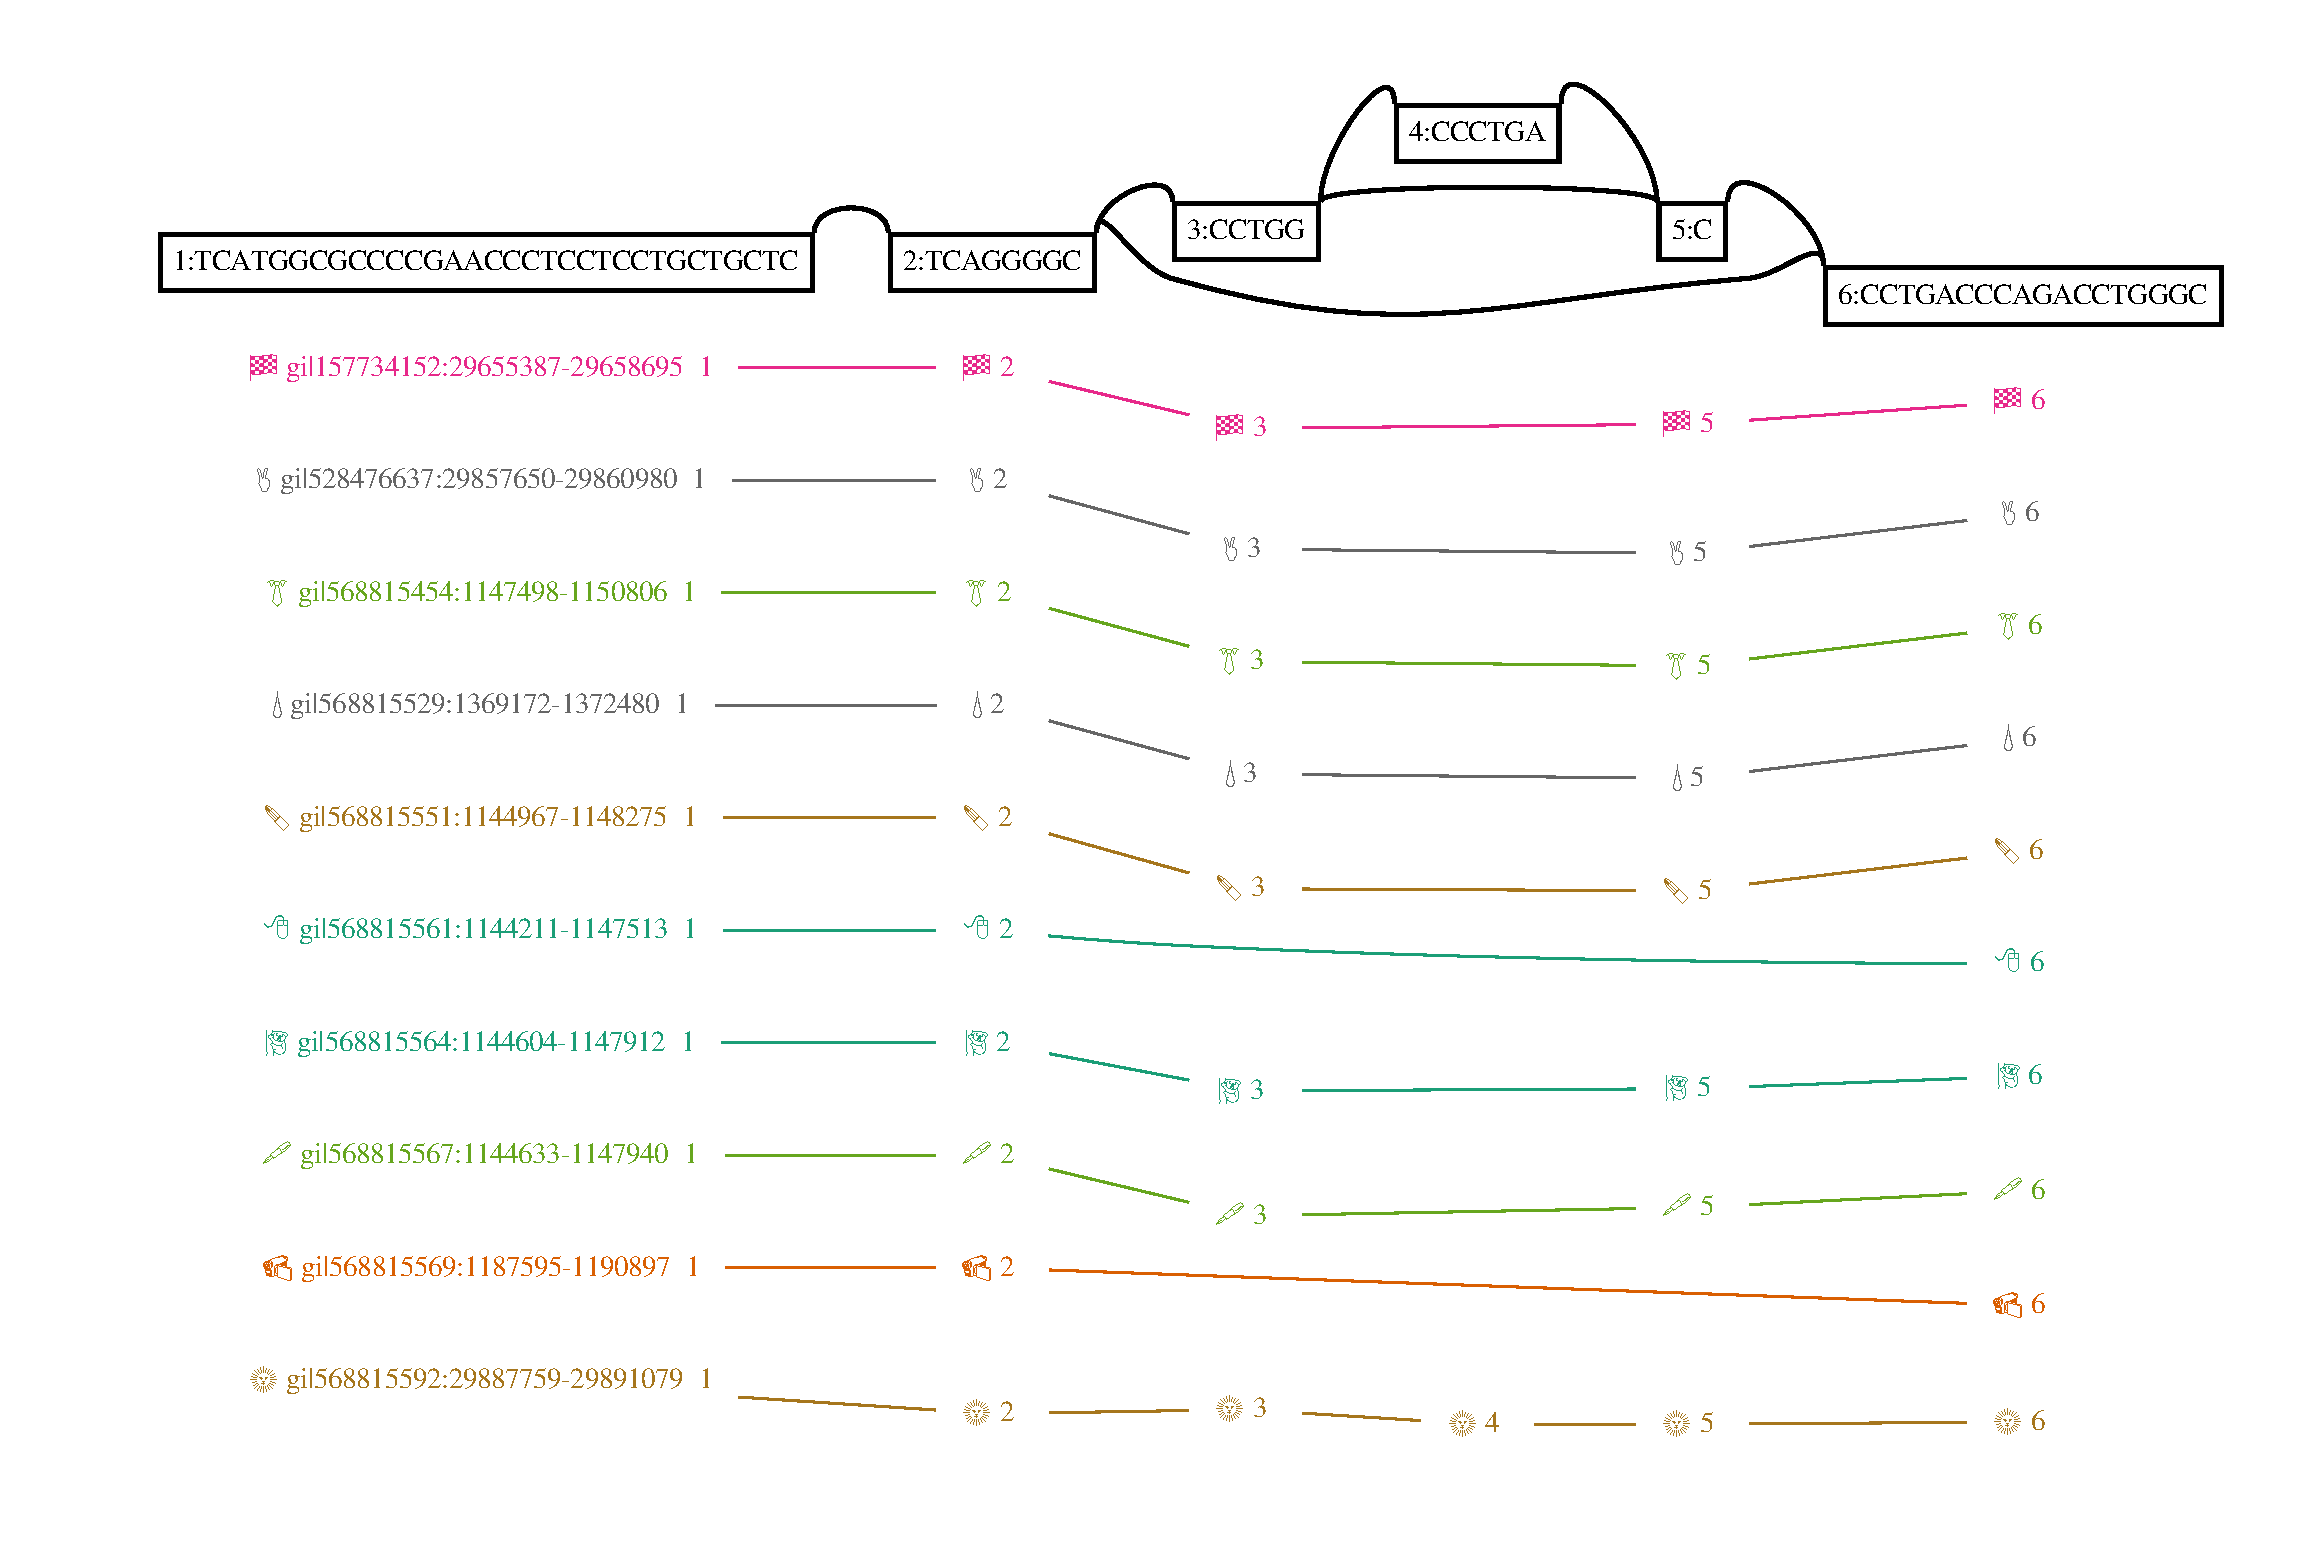
\includegraphics[width=1.0\textwidth]{Chapter2/Figs/vg_view_dp_H-3136_dot.pdf}
\caption[Hierarchical visualization with Graphviz's {\tt dot}]{The beginning of a variation graph built by progressive assembly of the GRCh38 haplotypes in HLA gene H-3136 visualized using {\tt dot}.}
\label{fig:vg_view_dot}
\end{figure}

\subsection{Force directed models}
%*1p 1.5h*

Not all graphs yield easily to hierachical layout algorithms.
Graphviz also includes a force-directed layout algorithm {\tt neato} that simulates the layout which would occur if connected nodes ``pull'' each other together and non-connected nodes ``repel'' each other apart.
While the same input to {\tt dot} may be used with {\tt neato}, in practice the node labels become impossible to read and the edge types are confusing to infer, so a simplified rendering is produced without specific sequence labels on the nodes.
This can still capture the overall structure of the graph as seen in figure \ref{fig:vg_view_neato}.

\begin{figure}[htbp!] 
\centering    
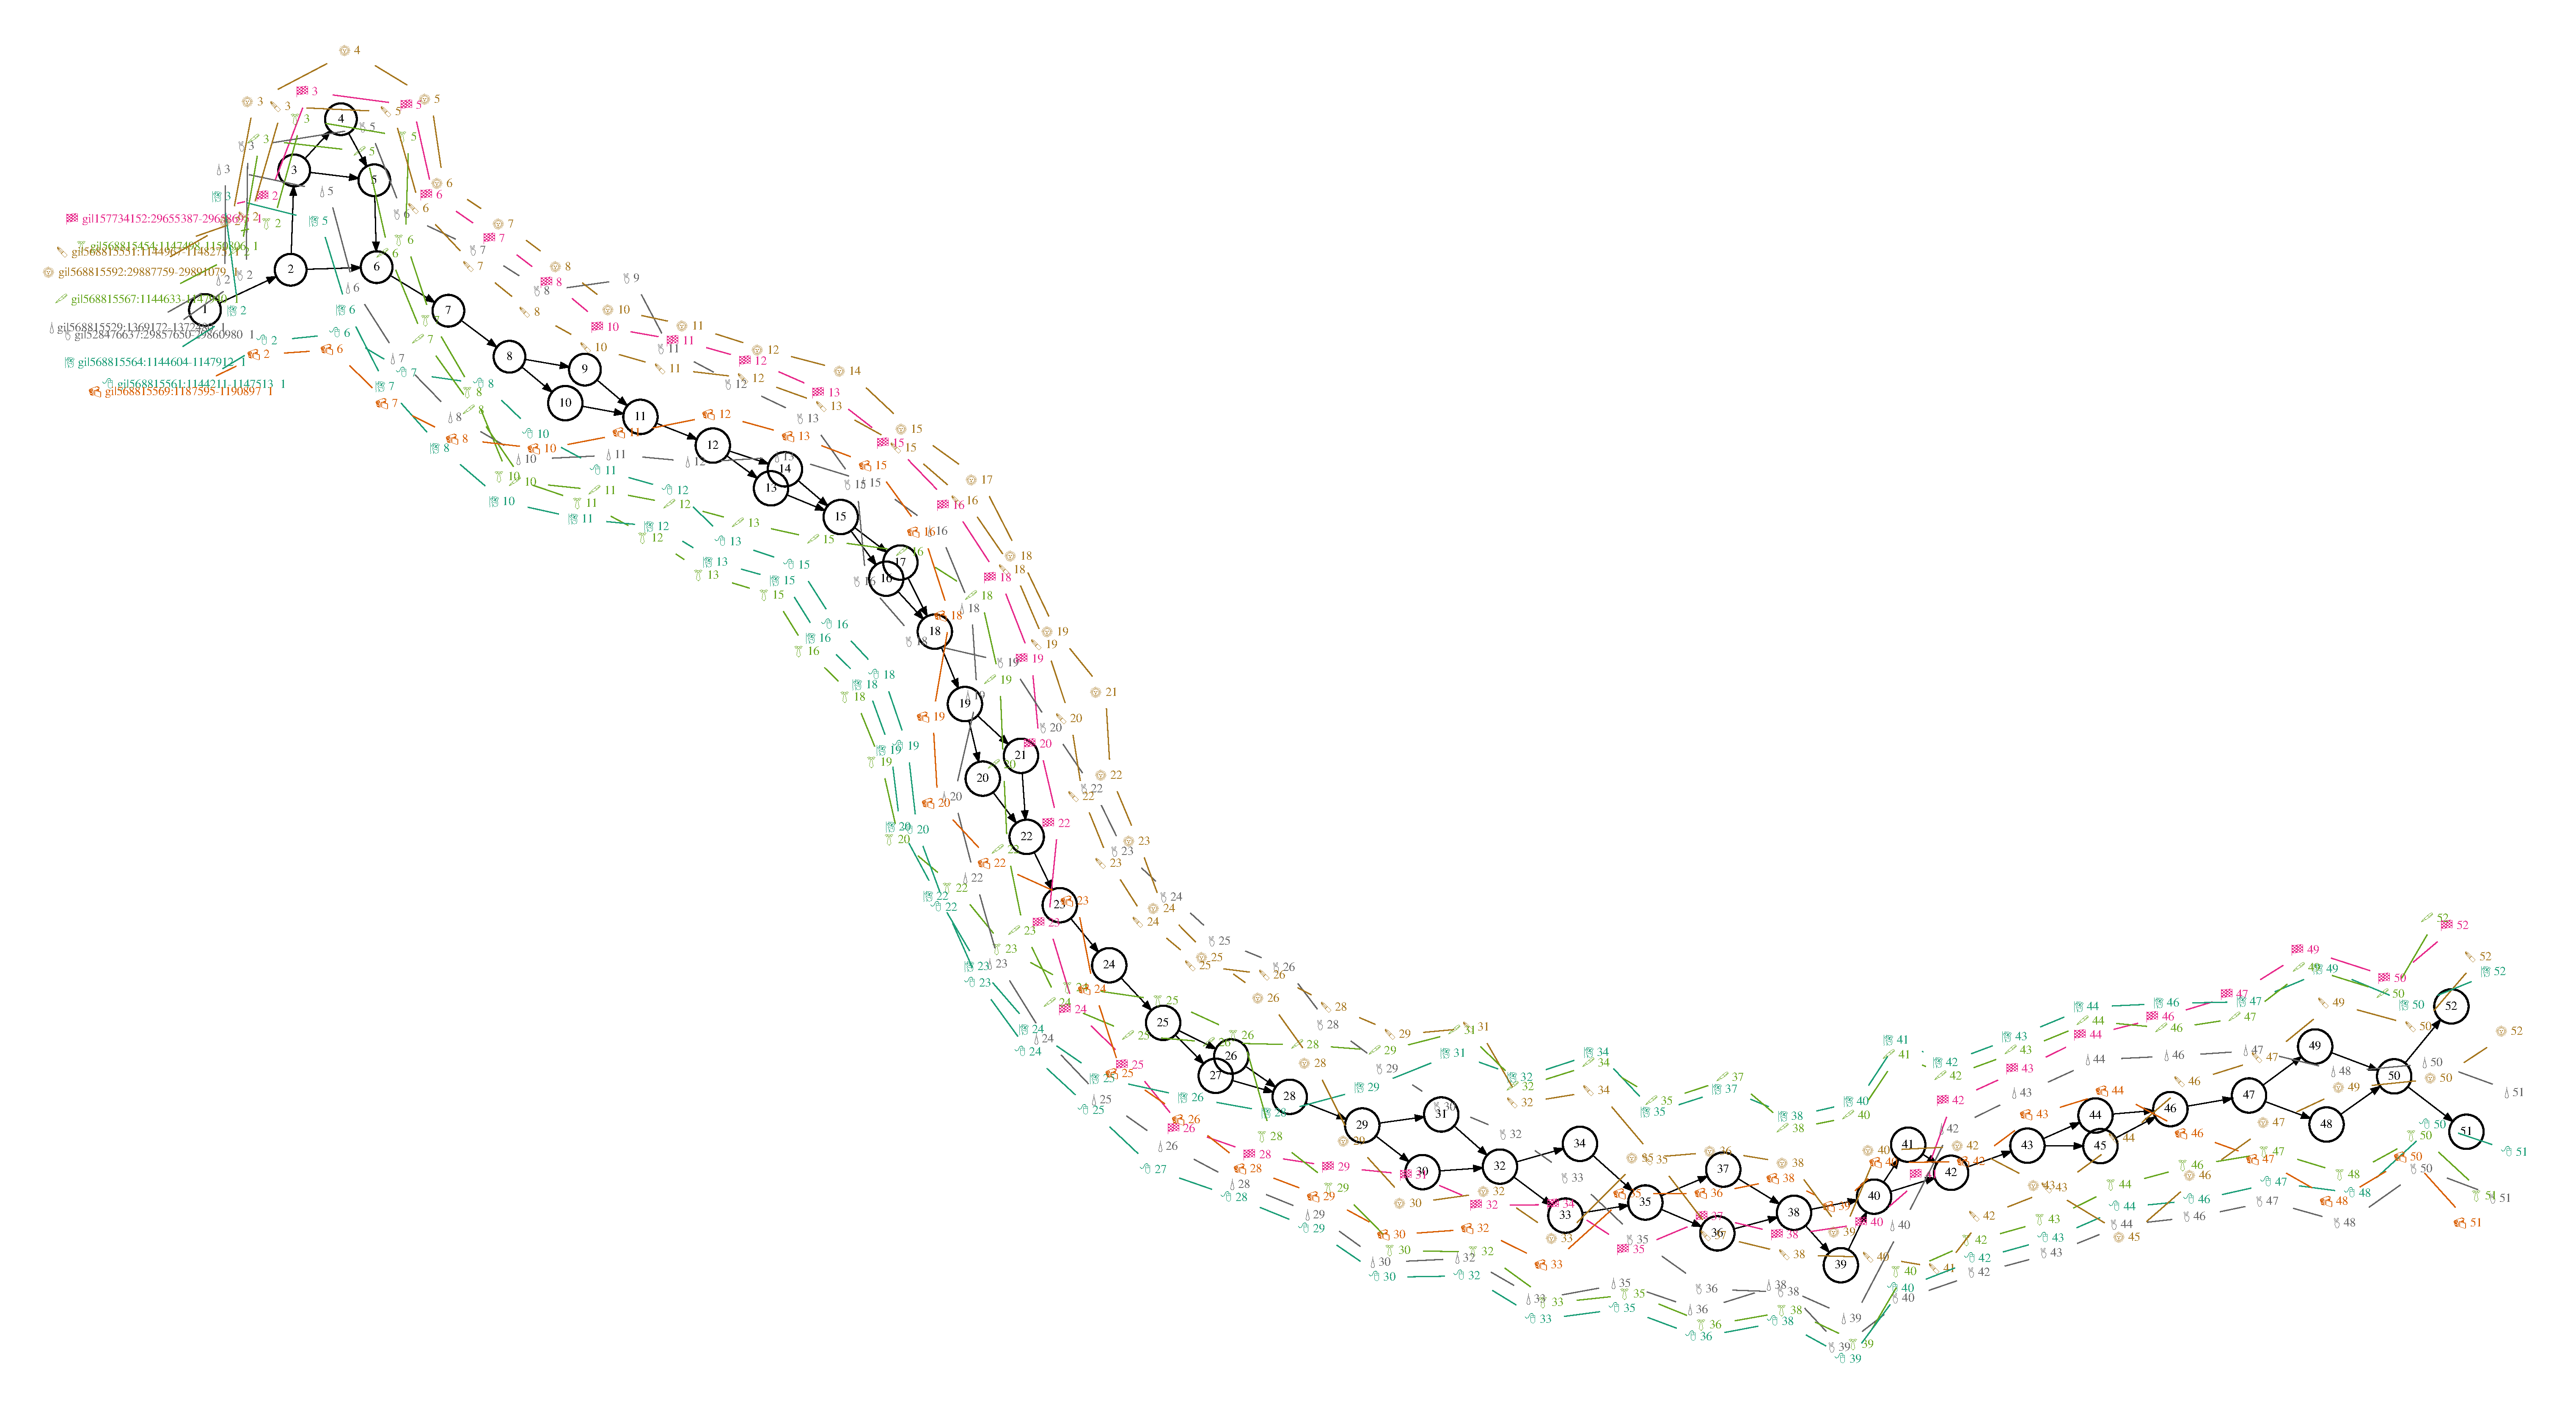
\includegraphics[width=1.0\textwidth]{Chapter2/Figs/vg_view_dpS_H-3136_neato.pdf}
\caption[Force-directed layout with Graphviz's {\tt neato}]{A larger region of the same variation graph in figure \ref{fig:vg_view_dot} rendered using {\tt neato}.}
\label{fig:vg_view_neato}
\end{figure}

While this rendering captures the path space of the graph even in arbitrary graphs, it cannot scale to graphs of significant size due to its approximately $O(|N|^3)$ scaling.
The largest graphs I have used this method to visualize contain tens of kilobases of sequence.
{\tt Bandage} \cite{wick2015bandage} is an alternative method which is oriented towards visualizing assembly graphs.
It reads GFA as input and provides an interactive rendering of the graph topology.
This assembly graph oriented approach allows for much better scaling for rendering variation graphs, and graphs of up to tens of megabases may be rendered.
Figure \ref{fig:vg_view_bandage} shows the properties of this technique using the same region of H-3136.

\begin{figure}[htbp!] 
\centering    
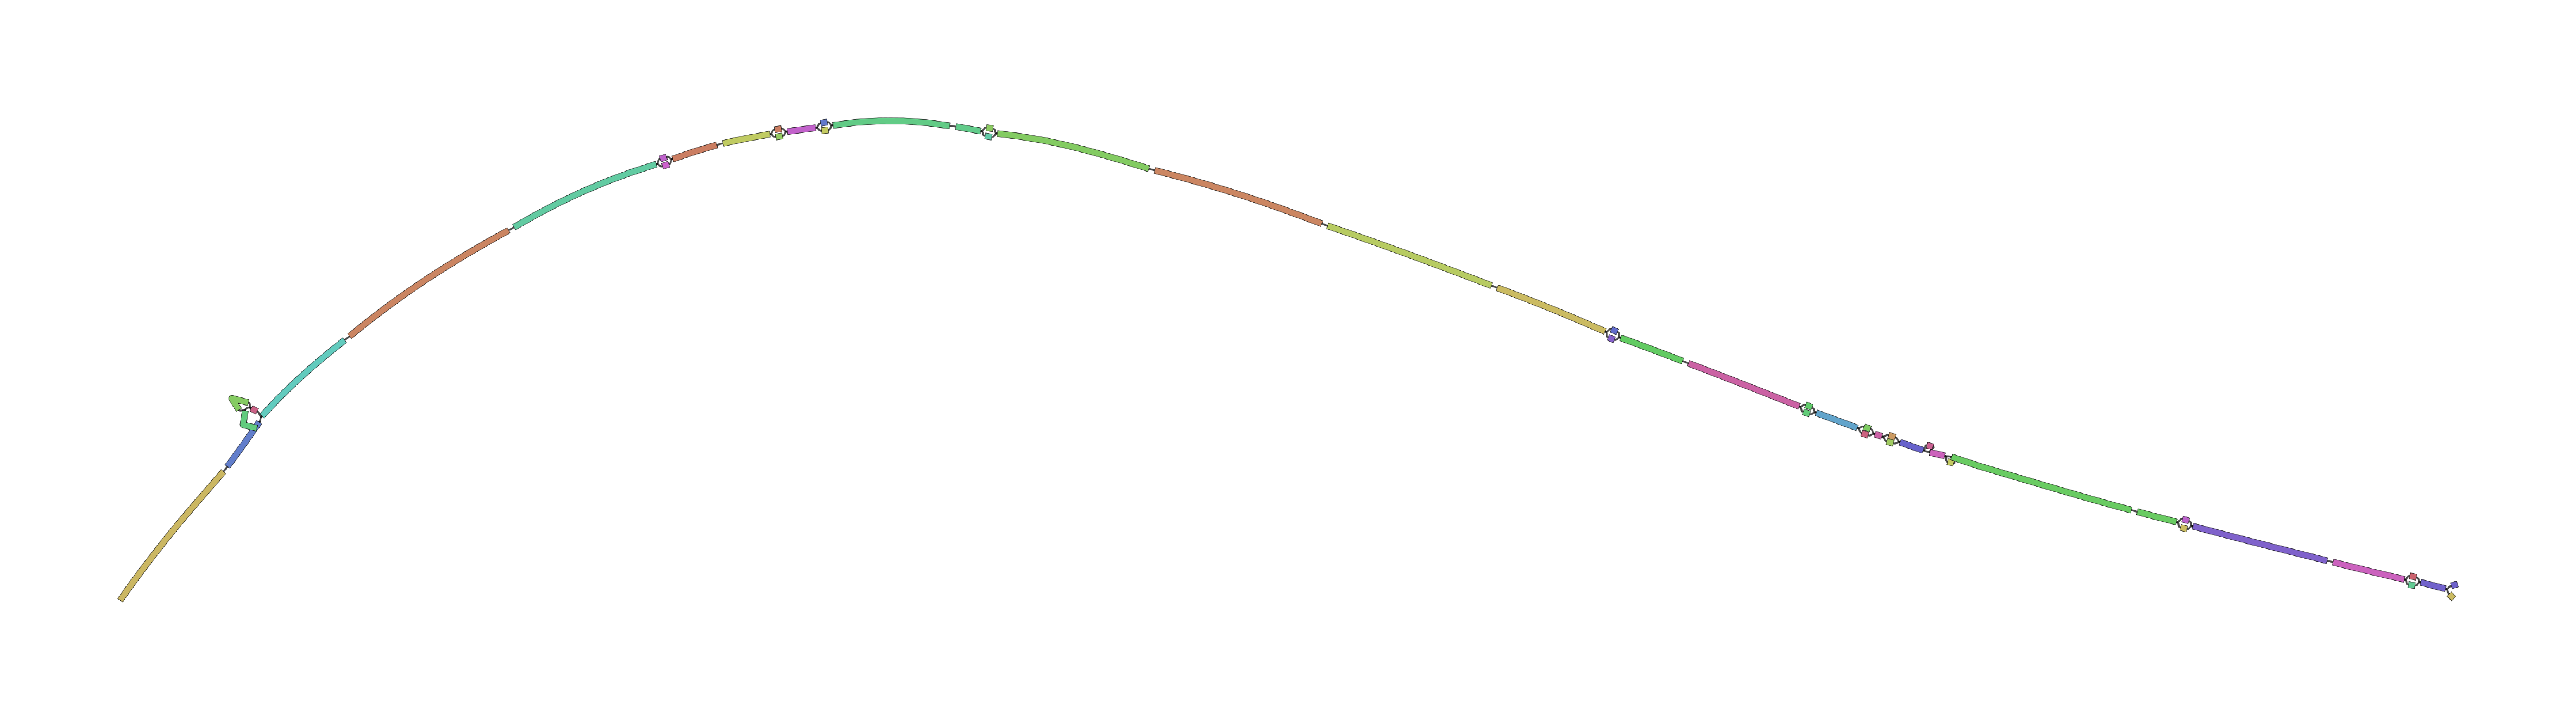
\includegraphics[width=1.0\textwidth]{Chapter2/Figs/vg_view_H-3136_Bandage.pdf}
\caption[Force-directed layout with Bandage]{The graph from figure \ref{fig:vg_view_neato} rendered using {\tt Bandage}.}
\label{fig:vg_view_bandage}
\end{figure}

\subsection{Linear time visualization}

Graph layout algorithms are computationally complex due to their need to iteratively relate all components of the graph to all others.
In these layouts, we can observe large scale features about the topology and organization of the graph.
These views are helpful in many contexts, but the computational complexity of obtaining them should not prevent us from quickly visualizing graphs as we can with linear sequences.
Furthermore, they do not scale efficiently to large path sets, and it is often difficult to understand alignments or other path-related on the graph using them.
Standard graph visualization algorithms exist outside of {\tt vg} as external tools.

To resolve these issues I developed a linear time rendering algorithm that projects a given VG, as indexed by XG, into a vector graphics format using the widely-available graphics library {\tt libcairo}.
The key idea is to use the sequence basis vector $S_\textbf{iv}$ as a coordinate system to position all elements of the graph.
The graph topology itself is laid out in accordance with the node representation in $S_\textbf{iv}$, flowing from left to right at the top of the rendering.
Node lengths are shown using a black bar, with the sequence labels given below.
The graph topology is rendered above the node set, and layout of these edges can be completed in linear time as they are rendered as simple splines connecting node ends.
Paths, or other annotations such as coverage per read set, are displayed below as colored bars matching the subset of the node space that they cover.
Where paths traverse a given node multiple times, an annotation is added to indicate the copy number.
This technique is implemented as {\tt vg viz}, and an example rendering is given in figure \ref{fig:vg_viz}.

\begin{figure}[htbp!] 
\centering    
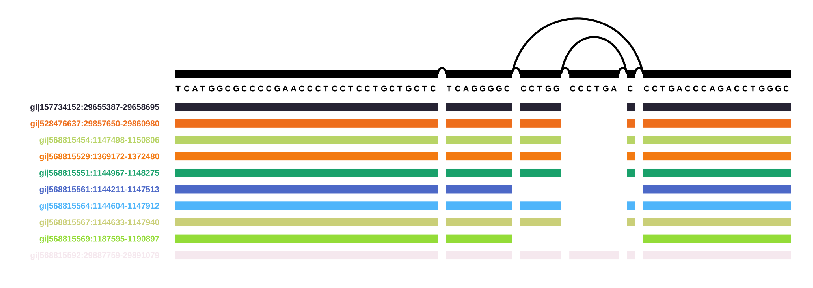
\includegraphics[width=1.0\textwidth]{Chapter2/Figs/vg_viz_H-3136.pdf}
\caption[Linearized variation graph visualization]{The same variation graph in figure \ref{fig:vg_view_dot} rendered using {\tt vg viz}.}
\label{fig:vg_viz}
\end{figure}

It is important to recognize that this approach is lossy.
Path ordering is not clearly represented, as the paths are treated like masks over the sequence space of the graph.
Furthermore, it can be difficult to interpret complex graphs as the topology of the graph is obscured in the simplistic rendering.
{\tt vg viz}'s linear layout treats the graph sequences as a basis space in which other paths or alignments may be interpreted.
This simplistic view is central to many potential applications of {\tt vg}, which I further discuss in section \ref{sec:basis_space}.
The linear scaling of the algorithm should allow it to be applied to whole genomes, provided suitable front-end visualization software can be built, such as in a web interface.

\section{Graph mutating algorithms}

Traversing the topology of the graph and querying its sequence space are important operations when using variation graphs as reference systems.
But to build these graphs, we need to be able to modify them.
Algorithms in graph theory are frequently based on graph transformations, and I have discussed some of them in the context of assembly and whole genome alignment.
{\tt vg} implements many algorithms that alter the graph, but a number are of importance to its development as a system for resequencing, and I detail them here.

\subsection{Edit}

As discussed in section \ref{sec:extending}, the extension of a variation graph to include new sequences and paths can be thought of as a transformation yielding a bijection between the new and old graphs $edit(G, A) \to (G', \Phi)$.
The particular implementation of this editing process is worth considering, as the variation graph data model has a number of particular features which add complexity to editing.
The main issue is that nodes represent more than a single character.

If nodes did represent a single character, then nodes are basically atomic through graph extension.
This approach is that used by POA.
It is simple to edit a ``basepair'' graph of this type: $G = (N, E, P) : |N| = \sum_{\forall n \in N} |seq(n)|$.
We walk through the alignments to it $A = a_1\ldots a_{|A|}$, adding novel bases represented by the alignment ($seq(A) \notin G = N_A$) as new nodes.
Then for each alignment $a_i$, we add edges connecting all of the nodes by edges in the order they would be traversed by the path of the alignment embedded in the graph $p_{a_i} \in G'$, yielding $E_A$.
Finally, we add paths representing the embedded alignments $P_A$.
The resulting graph unifies these additions $G' = (N \cup N_A, E \cup E_A, P \cup P_A)$.

To achieve lower representation costs in graphs with sparse variation, we compress the graph so that nodes may have $seq(n_i) > 1$ and thus we must consider the editing process hierarchically.
We first modify graph $G$ so that every novel sequence will be added at the start or end of a node.
We do this by breaking nodes into multiple derivative nodes when they overlap mappings that do not match the graph using $break(G, A) \to (G', \Phi)$.
For instance, if $seq(n_i) = {\tt GATTACA}$ and we have a SNP ${\tt T} \to {\tt C}$ at offset 4, we would obtain $n_i \to n_i', n_i'', n_i''' : seq(n_i') = {\tt GAT} \land seq(n_i'') = {\tt T} \land seq(n_i'') = {\tt ACA}$.
We can then apply $translate(A, \Phi) \to A'$, and add edges to $G'$ implied by the alignments as we would when editing a graph with single character nodes.

\subsection{Pruning}
%*2.5p 3h*

The number of paths in a sequence graph grows exponentially with the number of variable sites.
As I have discussed, this causes problems for alignment algorithms and graph sequence indexing.
While we can use efficient disk-backed index construction algorithms like GCSA2 to mitigate the effects of this exponential scaling, only a handful of dense clusters of variation in the graph can increase the memory requirements of path enumeration beyond any reasonable level.
Thus there is no reasonable choice but to restructure the graph to limit recombinations in the global sequence index.

We have explored two main techniques for the reduction of graph complexity.
In the first, we prune regions of the graph which have high path complexity using a depth-first search (DFS).
We can optionally add back known haplotypes, in order to mitigate the loss of information from the index.
For VCF-based VGs, where we have haplotype panels, the performance of local alignment is unaffected by the topological complexity, so we only need to apply this pruning to the graph input to GCSA2 indexing.
In assembly graphs, we find that some nodes which represent repeats can have extremely high degree, which causes problems both for indexing and local alignment to the graph.
There, we must remove these nodes in order to use the graph at all.

\subsubsection{$k$-mer ${\cal x}$-edge crossing complexity reduction}

In $k$-mer complexity reduction, we enumerate the $k$-mers of the graph, removing edges when a given $k$-mer crossing them would cross $\geq {\cal x}$ edges.
This can be done by creating a subgraph through a destructive complexity reduction filter, $prune(G, k, {\cal x}) \to G_\textbf{simple}$
We use the same $k$-mer enumeration algorithm that generates a DBG from the variation graph.
For each offest in each node $n_i$ and $\overline{n_i}$, we run a DFS forward until we have read $k$ characters of the graph.
During the pruning operation, instead of emitting the $k$-mers with their contexts, we stop the DFS when we have crossed ${\cal x}$ edges.
We record the edge in $E_\textbf{complex} = \{ e_{ij} : \exists p \in G |p| > {\cal x} \land node(p_{|p|-1} = i \land node(p_{|p|}) = j \}$.
We thus derive the subgraph from the current graph by removing the complexity-inducing edges: $(N, E \setminus E_\textbf{complex}, P) \to G_\textbf{simple}$.
It can be helpful to remove any short subgraphs that result from this pruning, which can be done with a linear subgraph enumeration algorithm and the measurement of the sequence length of each.
A subgraph $G_\textbf{sub} \in G_\textbf{simple} : \forall_{e_{ij} \in N_\textbf{sub}} n_i \in N_\textbf{sub} \land n_j \in N_\textbf{sub}$ must have length $\sum_{\forall n \in N_\textbf{sub}} |seq(n)| \geq {\cal J}$.
By default we use $k=24$, ${\cal x}=3$, and ${\cal J}=33$.

\subsubsection{Filling gaps with haplotypes}

Although removing complex regions will reduce the number of recombinant haplotypes represented by the graph, but it will also remove known haplotypes.
We can retain the complexity reduction without losing sequences in known haplotypes by replacing the pruned regions in $G_\textbf{simple}$ with unfolded copies of each haplotype sequence.
When we have a single reference path, we can accomplish this by overlaying $G_\textbf{simple}$ and $G_\textbf{ref}$.
However, this will not achieve the desired result with even two overlapping paths, as where these differ they would reintroduce the re-combinatorial explosion that we hope to resolve with pruning.
An alternative is to copy the haplotypes in the GBWT index that stretch from one border to the other of each removed region into the removed subgraphs in $G_\textbf{simple}$.
Doing so, we must preserve a mapping between the new nodes and the previous underlying ones in $G$.
This allows matches to the haplotypes to be converted into matches in the base graph.
The exact method by which this filling implemented is described in \cite{siren2018haplotype}.

\subsubsection{High degree filter}

As they separate dense variation into heterozygous bubbles, assembly graphs may feature greater ``smoothness'' than VCF-based graphs locally.
But, in the context of repeats, they can contain nodes with exceptionally high degree.
These highly-connected regions introduce degeneracy in the path space of the graph, and cause problems for $k$-mer enumeration and GCSA2 indexing.
Furthermore, the local alignment methods in VG do not directly support alignment through such dense regions.
This filter is relatively simple, in that we remove nodes with more than ${\cal D}$ edges linking them to the graph, yielding $G_\textbf{prune} : {\cal D} > |\{ e_{ij} \cup e_{ji} \cup e_{\overline{i}j} \cup e_{j\overline{i}} \} \forall i,j \in N_\textbf{prune}|$.

It is not necessary that our local alignment suffers from high-degree nodes.
The problem is that GSSW is provided an alignable graph that is an extracted subset of the full graph.
If this subgraph is extracted using context expansion in the graph, then high-degree nodes will generate extremely large subgraphs.
One solution would be to use the bit-parallel string to graph alignment approach in \cite{rautiainen2018bit}, as this achieves optimal bounds an the size of transformed graph to which we align.
Alternatively, the graph exploration should be more directly linked to the alignment process.
The X-drop aligner {\tt dozeu} could easily be adapted to this approach, as the X-drop parameter would provide a natural limit to the graph exploration.
Such approaches may allow us to tolerate a larger ${\cal D}$, but it seems unlikely that they will allow alignment to be driven through the most-tangled areas of the graph without a large performance penalty relative to graphs with lower maximum degree.

\subsection{Graph sorting}
%*1p 1h*

Order and orient the nodes in the graph using a topological sort.
The sort is guaranteed to be machine-independent given the initial graph's node and edge ordering.
The algorithm is well-defined on non-DAG graphs, but the order is necessarily not a topological order.
To do this we use a bidirected adaptation of Kahn's topological sort \cite{kahn1962topological}, which is extended to handle graph components with no heads or tails.
This algorithm can be understood as a kind of seeded depth first search through the graph.
Where the graph has nodes which are pure heads, it begins there
Otherwise, a set of seed nodes which are stably selected given a particular graph are used to begin the sort.
The details of this procedure are provided in algorithm \ref{alg:pseudotoposort}.

If the reference graph has been sorted, then we can use the given order to generate node identifiers.
These then allow us to efficiently sort subsets of the graph during read mapping.
The extracted subgraph may be sorted by id, and if $\exists e_{ij} : id(n_i) > id(n_j)$ then we know a cycle must exist.
The graph can then be passed to the DAGification procedure.
This allows us to avoid expensive sort operations during read alignment.

Similarly, the sort allows us to project data in the context of the graph into a single dimension.
Provided the graph is manifoldly partially ordered, this projection preserves local structures, which is a desirable property.
This makes the sort applicable to visualization techniques as in figure \ref{fig:vg_viz}.

\begin{algorithm}
  \caption[Pseudo-topological sort]{Pseudo-topological sort}
  \label{alg:pseudotoposort}
  \begin{algorithmic}
    \State $G = (N, E, P)$
    \Comment{A copy of our input graph which we will destructively modify}
    \State $L \gets [ \ldots ]$
    \Comment{Stores the pseudo-topological order}
    \State $S \gets \emptyset$
    \Comment{Set of nodes which have been oriented but not yet traversed}
    \State $V \gets \{ n_i \} \in N : \not \exists e_{ji} \forall n_j \in N$
    \Comment{We start from the head nodes of the graph}
    \If{$V = \emptyset$}
    \Comment{If there are no head nodes, we use ``seed'' nodes}
    \State $V \gets \text{Stably-selected seed nodes} \in N$
    \EndIf
    \While{$V \neq \emptyset$}
      \State $n \gets n \in V$
      \Comment{Select a seed node}
      \State $V \gets V \setminus \{n\}$
      \Comment{Remove it from the input node set $V$}
      \State $S \gets S \cup \{n\}$
      \Comment{Store it in our working set $S$}
      \While{$S \neq \emptyset$}
        \State $n_i \gets n_i \in S$
        \Comment{Remove an oriented node from $S$}
        \State $S \gets S \setminus \{n_i\}$
        \State $L \gets [L[1] \ldots L[|L|], n_i]$
        \Comment{Append it to our output order $L$}
        \For{$\forall n_j : e_{ij} \in E$}
          \State $E \gets E \setminus \{e_{ij}\}$
          \Comment{Remove the edge from our edge set}
          \If{$\not \exists e_{kj} \forall k \in N$}
          \Comment{$n_j$ has no other edges to that side}
          \If{$e_{i\overline{j}}$}
            \State $n_j \gets \overline{n_j}$
            \Comment{Orient $n_j$ so the side the edge comes to is first}
          \EndIf
          \State $N \gets N \setminus \{ n_j \}$
          \Comment{Remove $n_j$ from $N$}
          \State $S \gets S \cup \{ n_j \}$
          \Comment{Insert $n_j$ into $S$}
          \Else
          \Comment{This helps start at natural entry points to cycles}
            \State $V \gets V \cup \{ n_j \}$
            \Comment{Record $n_j$ as a place to start when $S$ is empty}
          \EndIf
        \EndFor
      \EndWhile
    \EndWhile \\
  \Return{$L$} \Comment{Return our pseudo-topologically sorted order and orientation}
\end{algorithmic}
\end{algorithm}
 

\subsection{Graph simplification}

Assembly algorithms often employ a \emph{bubble popping} phase, in which small bubbles, which are graph components connected to the rest of the graph through a single source and sink node, are replaced by linear components representing the most-likely path through the bubble given the read data.
In {\tt vg} we implement a similar technique based on the bubble decomposition of the graph.
Unlike assembly graph bubble popping, we must retain information about the embedded paths and annotations in the variation graph.
Simplification has a number of potential applications, for instance in reducing the complexity of visualizations of large variation graphs.

\section{Graphs as basis spaces for sequence data}
\label{sec:basis_space}

A reference genome allows us to interpret new sequences.
We can consider coverage over the reference genome, but this is incomplete because new sequences may contain variation that we have not seen.
Furthermore, the genome of the new sample may be diploid or polyploid, meaning the genomic state of the sample at a given locus is not trivially expressed as a single sequence.
This leads to the need for variant calling against linear reference genomes.

These steps do not change when our reference is a variation graph, but the scope in which they are relevant may be adjusted to meet our analysis needs.
If we can construct a graph which embeds all of the sequences of all genomes which we are interested in, then all sequences in our study are represented in the sequence space of the graph.
This resolves the separation between reference sequence and variation that is present in standard resequencing.
It also suggests that the intermediate steps in resequencing may be made redundant.
If variation is already available during alignment then there is no need for a variant detection phase.

However, if the graph does not include variation in our samples, then variant calling is required.
In {\tt vg} we have implemented several methods to do so.
Similarly, we have implemented coverage transformations of read sets that may be used directly in downstream analyses.

\subsection{Coverage maps}

Numerous population genetic analyses are based on matrix transformations of a collection of genomes.
Such models can be used to infer population structure and phylogeny, as well as to associate phenotypes to features in the genome such as causative variants.
If the variation graph used as a reference contains all sequences relevant to our anaylsis, then a matrix of per-base coverage of the graph by sample will provide nearly-full information to downstream analyses.
We cannot observe structural variation that does not result in coverage changes, such as balanced events like inversions.
Also, some local patterns of variation between successive small variation will not be differentiable.
If we were to annotate edge coverages, this method would produce a result equivalent in information content to a markov model.
It is thus clear that any coverage based index will be lossy relative to the full read set.
However, the lossiness reduces the information cost of storing and processing these coverage maps.
As I described in section \ref{sec:coverage_index}, in {\tt vg} I developed an efficent method to accumulate coverage information of this kind across the graph, but I have limited experimental results describing its utility.

\subsection{Bubbles}

In a sequence graph, a \emph{bubble} is a pair of paths which start and end at the same nodes ($s$, $t$) but are otherwise disjoint in the graph \cite{zerbino2008velvet}.
Bubbles encompass our intuition about genetic variation in graphs.
A homologous sequence corresponding to the common start and end nodes in the bubble flanks two or more alternative alleles in the middle.
These structures were first considered only in the process of finding small variation, and it was only in recent years that methods were developed to efficiently enumerate all bubbles of any size in DAGs \cite{birmele2012efficient}.

Bubbles can nest and contain more complicated internal structures between the paths through them.
The bubble may be generalized to the idea of a \emph{superbubble}, which is a directed, acyclic component of a graph with a single head and tail node \cite{onodera2013detecting}.
As for bubbles, efficient enumeration of superbubbles is possible in a DAG \cite{brankovic2016linear}.
The optimal method relies on a recursive topological sort of the graph to structure the nested bubbles.
Candidate node starts ($s$) and ends ($t$) are found following the definition of a superbubble.
The set of candidates is then validated by range min queries (RMQ) to produce the set of superbubbles.
As sort is linear $O(|N| + |E|)$, and the candidate enumeration and RMQ may be implemented on the sorted graph in $O(1)$ each, this yields a linear time algorithm for the enumeration of superbubbles.

The DAG requirement of this method is a significant limitation as it prevents us from directly applying the bubble finding to an arbitrary graph.
In order to apply the superbubble enumeration to a graph we must first DAGify it.
In response, along with Benedict Paten and others, I worked to further generalize the idea of a genetic site to work on arbitrary bidirectional sequence graphs \cite{paten2018superbubbles}.
To formulate a generalization of superbubbles, we introduce the concept of a \emph{snarl}, which is any graph component connected to the rest of the graph by less than two bordering nodes\footnote{In the paper the formulation is based on a biedged graph akin to the Enredo graph, but as we note a node-based formulation is equivalent and matches the other models in this section.}.
Snarls whose internal separated component are acyclic and do not contain any tips are \emph{ultrabubbles}.

Paten observed that trees embedded in the Cactus graph transformation of a variation graph corresponded to the standard concept of superbubbles.
Specifically, the cactus graph is transformed into a \emph{cactus tree} in which each simple cycle in the cactus graph becomes a special kind of node.
Various rootings of this tree may then be used to define a hierarchy of bubbles.
The bidirectional nature of the variation graph mean that snarls can embed each other in a manner akin to how the twist used to generate a M\"{o}bius strip results in it having a single surface and border.
In these cases the resulting cactus tree will support multiple ultrabubble tree rootings, and so unlike the bubble and superbubble decompositions for DAGs the ultrabubble decomposition is not complete.
We can enumerate a subset of these by identifying bridge edges (typically representing tips) in the ``bridge forest'', which is the result of a contraction of the cycles in the cactus graph into a set of top-level cycle representing nodes, and then use them to produce various rootings of the cactus tree.

Ultrabubbles and superbubbles provide a complete framework in which to reason about the hierarchy of variable genetic sites embedded in a graph.
As such they provide the basis for generic models of genotype inference based on variation graphs which are capable of genotyping any kind of genetic variation, including structural variation as well as nested variation in the same model as SNPs and indels.

\subsection{Variant calling}

Given a definition of variable genetic loci in the graph, we can build a genotyping system capable of generating genotype calls in the context of the graph.
In {\tt vg} we have explored two such methods.
The first, originally implemented in {\tt vg call}, generalizes the concepts first implemented in {\tt samtools mpileup} to work on the graph.
A set of alignments are first reduced to pointwise edits against the graph and per base coverage of the graph.
This graph ``pileup'' is then processed by a genotyping algorithm that considers genetic sites using the ultrabubble model.
The second model, implemented in {\tt vg genotype}, embeds the alignments in the variation graph using $edit(A, G_\textbf{base}) \to (G_\textbf{aug}, \Phi_{\textbf{aug}\to\textbf{base}})$, and then genotypes across the ultrabubbles of $G_\textbf{aug}$ which are supported by reference paths in $G_\textbf{base}$ or reads.
As the resulting genotypes are represented as unordered sets of paths in $G_\textbf{aug}$, they are projected back into the coordinate space of $G_\textbf{base}$ using the translation $\Phi_{\textbf{aug}\to\textbf{base}}$.

While principled, the full augmentation model in {\tt vg genotype} is very expensive to compute.
The pileup model has proven to be more efficient.
Over time {\tt vg call} has been adjusted to implement a variant of the full graph augmentation model in {\tt vg genotype} where the graph is augmented only with sequences supported by some number of alignments at a given quality threshold.
Both methods employ a diploid specification of the genotyping model in freebayes \cite{garrison2012haplotype} to develop their posterior estimates of variant quality.
The generalization of SNP and indel calling to haplotype calling implemented in freebayes corresponds to the same allele model used in both {\tt vg} variant calling methods.
In all alleles correspond to DNA sequences of arbitrary length, anchored at the ends to the reference genome (in the case of freebayes) or to the rest of the graph (as in the ultrabubbles used in {\tt vg}).

The complexity of running genotyping in the graph has slowed development of these methods.
Currently they are outperformed by standard variant calling methods based on the linear reference, as indicated by our results in the PrecisionFDA variant calling challenge that I will describe in the next chapter.

%\subsection{MEM matching to the bidirectional GBWT}

\section{Contributions to related computational methods}

% in this chapter I've described things that I've done
% as a consequence of being in this work, here are things that I helped other people to build
% list papers, give references

% gpBWT
% GCSA2
% ...
